\documentclass[runningheads]{llncs}

\usepackage[T1]{fontenc}
\usepackage{graphicx}
\usepackage{amsmath,amssymb}
\usepackage{booktabs}
\usepackage{float}
\usepackage{multirow}
\usepackage{placeins}
\usepackage{wrapfig}
\usepackage{tikz}
\usetikzlibrary{decorations.pathreplacing,calc}

\newcommand{\method}{JSQKV}
\newcommand{\attnscorefigdir}{figures/attnscorecrossfigdir}
\newcommand{\attnscorecrossfigdir}{figures/attnscorecrossfigdir}
\newcommand{\multifieldqa}{Multi\-FieldQA-EN}
\newcommand{\multifieldqaheader}{\shortstack{MultiFieldQA-\\EN}}

\newif\ifanonymous
% \anonymoustrue
\anonymousfalse % Uncomment for the camera-ready version.

\ifanonymous
\newcommand{\paperauthors}{Anonymous Authors}
\newcommand{\paperauthorrunning}{Anonymous Submission}
\newcommand{\paperinstitute}{Anonymous Institution}
\newcommand{\paperavailability}{Code repository omitted for double-blind review.}
\else
\newcommand{\orcidHaoZhang}{\orcidID{0009-0001-1044-0312}}
\newcommand{\orcidXiaoliGong}{\orcidID{0000-0002-9836-558X}}
% \newcommand{\orcidHaoranLi}{\orcidID{0009-0001-1044-0312}}
% \newcommand{\orcidHuayouSu}{\orcidID{0009-0001-1044-0312}}
% \newcommand{\orcidQingxiaChen}{\orcidID{0009-0001-1044-0312}}
\newcommand{\orcidJinZhang}{\orcidID{0000-0001-9086-1178}}
\newcommand{\paperauthors}{%
Hao Zhang\inst{1}\orcidHaoZhang \and
Xiaoli Gong\inst{1}\orcidXiaoliGong\textsuperscript{*} \and
Haoran Li\inst{1} \and
Huayou Su\inst{2} \and
Qingxia Chen\inst{3} \and
Jin Zhang\inst{1}\orcidJinZhang}
\newcommand{\paperauthorrunning}{H. Zhang et al.}
\newcommand{\paperinstitute}{%
College of Computer Science, Nankai University, Tianjin, China\\
\email{\{2120230710, gongxiaoli, wanch\_lhr, nkzhangjin\}@nankai.edu.cn}
\and
National University of Defense Technology, Changsha, China\\
\email{shyou@nudt.edu.cn}
\and
Qian Xuesen Laboratory of Space Technology, Beijing, China\\
\email{chenqingxia\_0882@163.com}}
\newcommand{\paperavailability}{Code is available at \url{https://github.com/Haozon/JSQKV}.}

\fi

\begin{document}

\title{\method: Joint Sparsification and Quantization for KV-Cache Compression and Decode Acceleration}
\titlerunning{\method\\: Joint Sparsification and Quantization for KV-Cache Compression}

\author{\paperauthors}
%
\authorrunning{\paperauthorrunning}
% First names are abbreviated in the running head.
%
\institute{\paperinstitute}

\maketitle
\begin{abstract}

% As long-context large language models become increasingly widespread, autoregressive decoding is increasingly bottlenecked by KV-cache footprint and memory bandwidth. Existing KV-cache compression methods typically rely on sparsification or low-bit quantization, but simply combining the two often fails to simultaneously preserve model accuracy and deliver real system-level gains.
As long-context large language models become increasingly widespread, autoregressive decoding is increasingly bottlenecked by KV-cache footprint and memory bandwidth. Existing KV-cache compression methods typically rely on sparsification or low-bit quantization, but simply combining the two often fails to simultaneously preserve model quality and deliver real end-to-end speedup, since sparsification changes how compressed KV-cache states are represented and executed during decoding.
% We present \method\, a joint sparse-quant framework for KV-cache compression and decode acceleration that co-desigins compression policy, numerical representation, and execution path. \method\ introduces an attention-score-based differential sparsification strategy with a dual-window online execution mechanism, together with a Hadamard-based Per-Token-Tile quantization scheme and a bitmap-based sparse-quant format with a matching decode kernel. This co-design enables compressed KV-cache data to remain compact in memory while being effectively translated into reduced memory traffic and end-to-end speedup.
% 我们联合设计的是：压缩决策 → 压缩后表示/格式 → 执行路径。
To address this issue, we present \method\, a joint sparse-quant framework for KV-cache compression and decode acceleration that co-designs compression policy, compressed format, and execution path. Specifically, \method\ combines attention-score-based differential sparsification with a dual-window online mechanism, Per-Token-Tile quantization with Hadamard rotation, and a bitmap-based sparse-quant format with a matching decode kernel. Through this joint design, compressed KV-cache data remains compact in memory and is more effectively translated into reduced memory traffic and end-to-end speedup.
% Experimental results show that, under matched compression budgets, \method\ generally outperforms the sequential MUSTAFAR+KIVI baseline on LongBench, with larger gains under more aggressive sparse-quant settings. On Llama-3-8B, \method\ improves end-to-end throughput by 44.2\% over dense decoding in a long-context setting, while increasing the KV-cache compression ratio to 3.48$\times$. These results support jointly optimizing compression policy, numerical representation, and execution path for efficient KV-cache compression.
Experimental results show that, under matched compression budgets, \method\ generally outperforms the sequential MUSTAFAR+KIVI baseline on representative LongBench tasks, with larger gains under more aggressive sparse-quant settings. On Llama-3-8B-Instruct, \method\ improves the average score on six representative LongBench tasks from 39.83 to 43.12, while also improving end-to-end throughput by 44.2\% over dense decoding and increasing the KV-cache compression ratio to 3.48$\times$.
% \paperavailability
% Experimental results show that, under matched compression budgets, \method\ generally compares favorably with the sequential MUSTAFAR+KIVI baseline on LongBench, with larger gains under more aggressive sparse-quant settings. On Llama-3-8B-Instruct, with input length 4096 and output length 256, \method\ improves end-to-end throughput by 44.2\% over the dense baseline at batch size 4 using 70\% KV sparsity and 2-bit quantization, while increasing the KV-cache compression ratio to 3.48$\times$. These results suggest that efficient KV-cache compression benefits from joint optimization across compression policy, numerical representation, and execution path. \paperavailability

\keywords{KV-cache compression \and Sparsity \and Quantization}
\end{abstract}

\section{Introduction}
\label{sec:intro}

As context windows continue to grow in large language models, autoregressive decoding is increasingly bottlenecked by KV-cache footprint and memory bandwidth~\cite{ding2024longrope}. Since the KV cache grows linearly with context length and is repeatedly accessed during decoding, this stage is more memory-bound than prefill and increasingly limits throughput, batch size, and deployment efficiency in long-context settings~\cite{kwon2023pagedattention,agrawal2024sarathiserve}.

Prior work on KV-cache compression mainly follows two directions: sparsification and low-bit quantization. Token eviction and sparsification reduce retained history or prune redundant KV states~\cite{xiao2024streaming,zhang2023h2o,snapkv,pyramidkv,xu2025think,lv2024kvpruner,joo2025mustafar}, while quantization lowers the numerical precision of retained cache elements~\cite{liu2024kivi,hooper2024kvquant,ashkboos2024quarot,chen2025rotatekvaccuraterobust}. Although both are effective, existing studies still largely treat them as separate components.

In practice, joint sparse-quant KV-cache compression is not a simple sparse-then-quantize pipeline. Sparsification changes not only how much KV data is kept, but also the retained token and feature layout, which in turn affects quantization granularity, compressed data layout, and decode-time execution. As a result, algorithm-level compression gains do not automatically translate into lower memory traffic or real end-to-end speedup during decoding~\cite{agrawal2024sarathiserve,zhong2024distserve,joo2025mustafar}. Moreover, token-differential compression is easy to estimate in prefill, where future attention is observable, but difficult to apply online during autoregressive decoding, where a token must be cached before its future importance can be known. Thus, the key challenge is twofold: preserving model quality under aggressive compression and keeping the compressed representation directly executable for practical decode-time acceleration.

\begin{figure}[t]
\centering
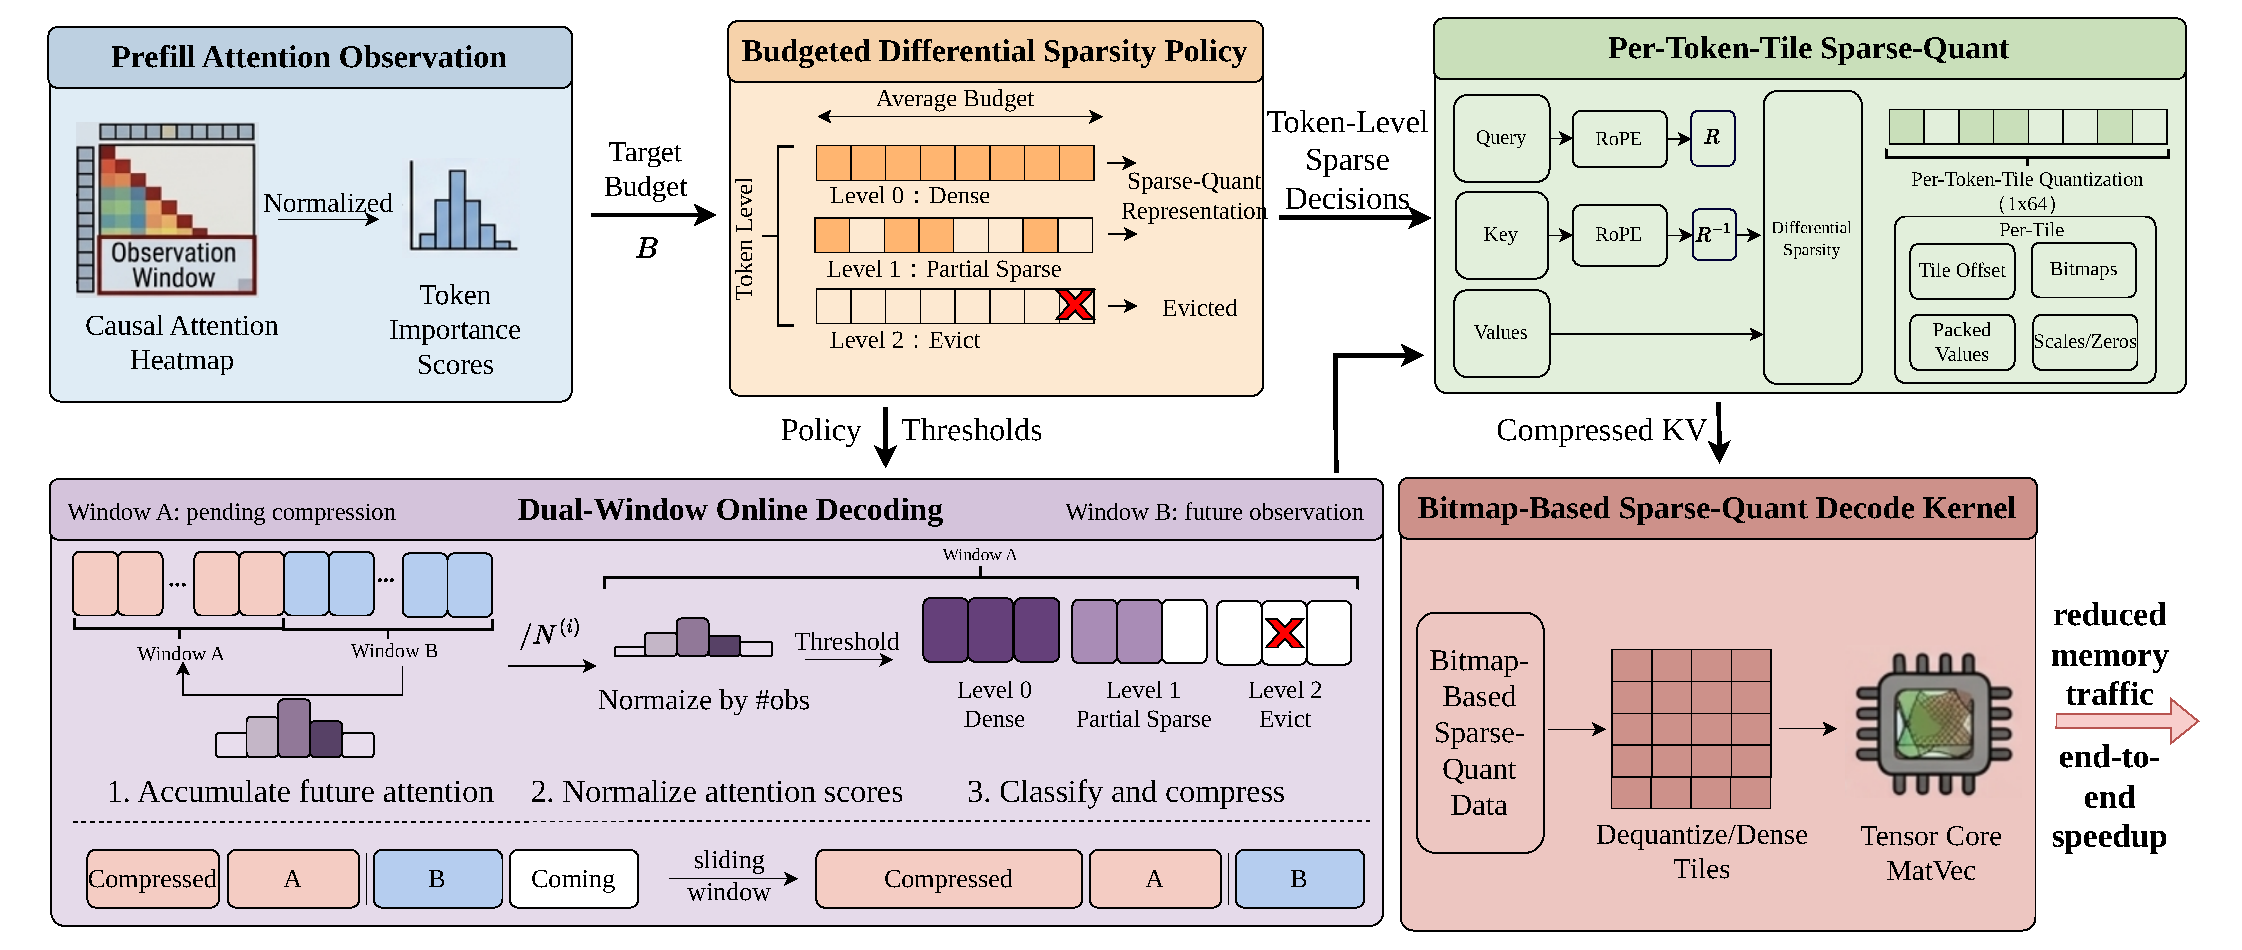
\includegraphics[width=0.96\linewidth]{figures/JSQKV_Overview.drawio_pdf14.pdf}
\caption{Overview of \method. The framework combines differential sparsity, dual-window online execution, Per-Token-Tile quantization with Hadamard rotation, and a bitmap-based sparse-quant decode path.}
\label{fig:JSQKV-overview}
\end{figure}
To address these challenges, we propose \method, a joint sparse-quant framework for KV-cache compression and decode acceleration. Rather than treating sparsification and quantization as separate post-processing steps, \method\ co-designs compression policy, compressed representation, and runtime execution in a unified decode-stage pipeline, as illustrated in Fig.~\ref{fig:JSQKV-overview}. Section~\ref{sec:diff-sparsity} introduces an attention-score-based differential sparsification policy that allocates different compression budgets to historical tokens according to estimated future importance. Since such token-differential decisions are easy to estimate in prefill but not directly available when tokens are generated online, Section~\ref{sec:dual-window} presents a dual-window mechanism that accumulates future observations before compression and makes the differential policy applicable during autoregressive decoding. After sparse decisions are made, the remaining KV states still require a low-bit representation that is both robust and compatible with token-level sparse execution. To this end, Section~\ref{sec:quant} introduces Hadamard-based Per-Token-Tile quantization to mitigate key outliers and align quantization granularity with downstream computation. Finally, Section~\ref{sec:sparse-quant} presents a bitmap-based sparse-quant format and a matching decode kernel that keep the KV cache compact in memory and convert compression savings into reduced memory traffic and practical end-to-end decoding speedup. Together, these components form a unified sparse-quant decode pipeline for accurate and efficient KV-cache compression, and our evaluations show that \method\ compares favorably with sequential sparse-quant baselines while also delivering practical end-to-end decoding speedup.

The main contributions of this paper are as follows:
\begin{itemize}
    \item We propose an attention-score-based differential sparsification policy that assigns different sparsity levels to historical tokens under a fixed average compression budget, instead of applying a uniform compression ratio to all tokens.
    \item We design a dual-window online execution mechanism that makes this differential policy usable in autoregressive decoding, where future attention evidence is unavailable when a token is first generated.
    \item We propose Hadamard-based Per-Token-Tile quantization for the retained KV states to stabilize low-bit representation and align quantization granularity with token-level compression decisions.
    \item We design a bitmap-based sparse-quant format and matching decode kernel so that compressed KV-cache representations can be translated into reduced memory traffic and practical decode-time speedup.
\end{itemize}

% Overall, prior work shows that both sparsification and quantization are effective, but the two are still largely studied in isolation. In practice, joint compression is not a simple sequential combination: sparsification determines which token states or features are removed, while quantization determines how the remaining nonzero states are represented. Once sparsification changes the retained tokens and cache access pattern, the appropriate quantization granularity, compressed data layout, and decode-time kernel design also change. Without such co-design, algorithm-level compression gains may not reliably translate into practical end-to-end speedups~\cite{agrawal2024sarathiserve,joo2025mustafar}.

% To address this issue, we propose \method, a joint sparse-quant framework for KV-cache compression and decode acceleration. \method\ jointly designs compression policy, numerical representation, and execution path. A key challenge is that token-differential compression is easy to estimate in prefill, but not directly usable at decode time, where future attention evidence is unavailable when a token is first generated. The key idea is simple: allocate different compression budgets to different tokens according to their importance to future attention, compress the remaining KV states with a token-aligned and numerically stable low-bit representation, and keep the KV cache compressed in memory as much as possible until dense tiles are required by the decode kernel. Through this joint design, \method\ keeps the KV cache compact in memory while more effectively reducing memory traffic and improving end-to-end throughput.

% The main contributions of this paper are as follows:
% \begin{itemize}
%     \item We propose an attention-score-based differential sparsification policy that assigns different sparsity levels to different historical tokens at the token level, instead of applying a single global compression ratio.
%     \item We design a dual-window online execution mechanism for autoregressive decoding, extending differential sparsification from the prefill stage to online decoding.
%     \item We propose a Hadamard-based Per-Token-Tile quantization method to mitigate low-bit quantization instability caused by Key outliers and to better align quantization granularity with token-level compression decisions.
%     \item We design a bitmap-based sparse-quant format and a matching decode kernel that keep the compressed KV cache compact in memory and turn compression into reduced memory traffic and end-to-end decoding speedup.
% \end{itemize}

% The main contributions of this paper are as follows:
% \begin{itemize}
%     \item We propose an attention-score-based differential sparsification policy that assigns different sparsity levels to historical tokens under a fixed average compression budget, instead of applying a uniform compression ratio to all tokens.
%     \item We design a dual-window online execution mechanism that makes this differential policy usable in autoregressive decoding, where future attention evidence is unavailable when a token is first generated.
%     \item We propose Hadamard-based Per-Token-Tile quantization for the retained KV states to stabilize low-bit representation and align quantization granularity with token-level compression decisions.
%     \item We design a bitmap-based sparse-quant format and matching decode kernel so that compressed KV-cache representations can be translated into reduced memory traffic and practical decode-time speedup.
% \end{itemize}

% Experimental results show that \method\ achieves a favorable balance between model quality and system efficiency under high compression ratios. On Llama-3-8B-Instruct~\cite{grattafiori2024llama3}, with 70\% KV cache sparsity and 2-bit quantization, \method\ improves end-to-end throughput by approximately 44.2\% over the dense baseline in a long-context decoding setting with batch size 4. Under matched compression budgets, \method\ generally compares favorably with the sequential MUSTAFAR+KIVI baseline, with larger gains under more aggressive sparse-quant settings. These results support the motivation of treating KV-cache compression as a joint optimization problem across compression policy, numerical representation, and execution path.
\section{Background and Related Work}
\label{sec:bg_related}
\subsubsection{KV Sparsification}
KV-cache sparsification reduces memory cost by removing less useful history or pruning retained states during decoding. Token-level retention and eviction methods, such as StreamingLLM~\cite{xiao2024streaming}, H$_2$O~\cite{zhang2023h2o}, SnapKV~\cite{snapkv}, and PyramidKV~\cite{pyramidkv}, exploit the unequal contribution of historical tokens to future decoding. Finer-grained sparsification further explores redundancy within retained KV states. ThinK~\cite{xu2025think} prunes key channels using query-dependent importance, KVPruner~\cite{lv2024kvpruner} studies structured pruning of KV blocks, and MUSTAFAR~\cite{joo2025mustafar} shows that unstructured per-token sparsity can be practical when paired with a bitmap-based sparse format and a matching attention kernel.

\subsubsection{KV-Cache Quantization}
KVQuant~\cite{hooper2024kvquant} studies ultra-low-bit KV-cache quantization for long-context inference, KIVI~\cite{liu2024kivi} uses asymmetric quantization with different granularities for Keys and Values, and QuaRot~\cite{ashkboos2024quarot} and RotateKV~\cite{chen2025rotatekvaccuraterobust} improve low-bit robustness by reshaping activation distributions before quantization. These methods differ in quantization granularity, metadata cost, and execution compatibility.

\subsubsection{Systems and Kernels for Attention}
PagedAttention~\cite{kwon2023pagedattention} improves KV-cache management through block-based memory organization, while FlashDecoding~\cite{hong2024flashdecoding} and FlashInfer~\cite{ye2025flashinfer} optimize decode-stage attention in memory-bound settings. Loki~\cite{singhania2024loki} leverages low-rank keys to reduce data movement and computation, Flash-LLM~\cite{xia2023flashllm} supports unstructured sparsity on Tensor Cores through a load-as-sparse and compute-as-dense framework, and Coruscant~\cite{joo2025coruscant} further co-designs GPU kernels and sparse tensor cores for efficient unstructured sparse LLM inference.
\section{Method}
\label{sec:method}

% \subsection{Overview}
% \begin{figure}[t]OverOverviewview
% \centering
% 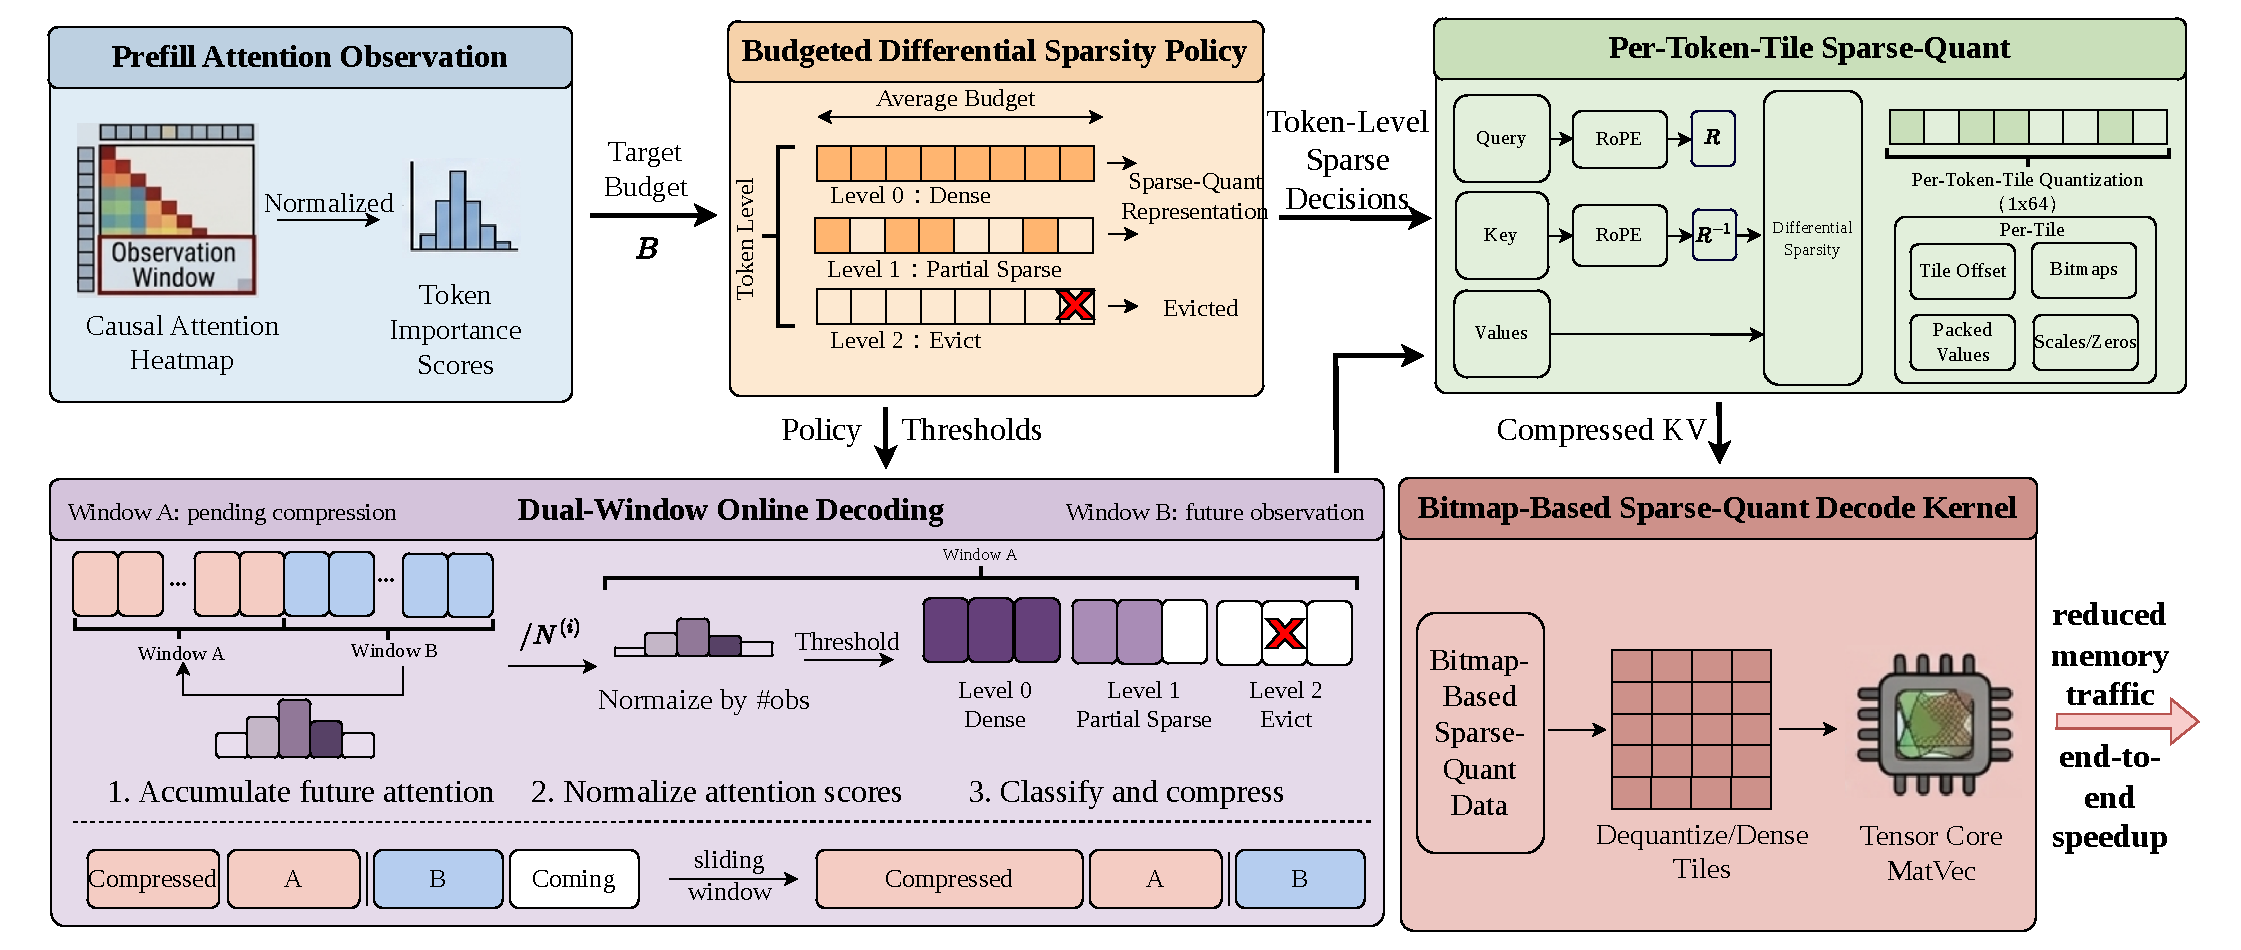
\includegraphics[width=0.96\linewidth]{figures/JSQKV_Overview.drawio.pdf}
% \caption{Overview of \method. The framework combines differential sparsity, dual-window online execution, Per-Token-Tile quantization with Hadamard rotation, and a bitmap-based sparse-quant decode path.}
% % \caption{Overview of \method\. The method first estimates token importance from prefill attention and instantiates a budgeted differential sparsity policy. It then extends this policy to autoregressive decoding through a dual-window online execution mechanism, represents retained KV states with Hadamard-based Per-Token-Tile quantization, and finally executes the compressed cache with a bitmap-based sparse-quant decode kernel to reduce memory traffic.}
% \label{fig:JSQKV-overview}
% \end{figure}

% % Figure~\ref{fig:JSQKV-overview} summarizes the overall design of \method. Rather than applying sparsification and quantization as two independent post-processing steps, \method\ organizes them into a unified decode-stage pipeline that jointly designs compression policy, low-bit representation, and execution path. The framework consists of four tightly coupled components: a budgeted differential sparsity policy estimated from prefill attention, a dual-window online mechanism that delays compression until enough future evidence has been accumulated, Hadamard-based Per-Token-Tile quantization for the retained KV states, and a bitmap-based sparse-quant format with a matching decode kernel that keeps the KV cache compact in memory and translates compression into reduced memory traffic and practical decode-time speedup.

% Figure~\ref{fig:JSQKV-overview} summarizes the overall design of \method. A naive sparse-then-quantize pipeline is insufficient for decode-stage KV-cache compression. The reason is that sparsification changes not only how much KV data is kept, but also which tokens and features remain nonzero. This in turn changes the appropriate quantization granularity, compressed layout, and decode-time execution path. If these components are designed independently, the compressed cache may achieve a smaller nominal footprint yet still fail to reduce memory traffic or deliver practical end-to-end speedup during decoding. In addition, token-differential compression is easy to estimate in prefill but difficult to apply online, because future attention evidence is unavailable when a token is first generated during decode.

% To address these issues, \method\ organizes sparsification, quantization, and execution into a unified decode-stage pipeline. The framework consists of four tightly coupled components: a budgeted differential sparsity policy estimated from prefill attention, a dual-window online mechanism that delays compression until enough future evidence has been accumulated, Hadamard-based Per-Token-Tile quantization for the retained KV states, and a bitmap-based sparse-quant format with a matching decode kernel that keeps the KV cache compact in memory and translates compression into reduced memory traffic and practical decode-time speedup.

% Figure~\ref{fig:JSQKV-overview} summarizes the overall design of \method. Rather than applying sparsification and quantization as two independent post-processing steps, \method\ organizes them into a unified decode-stage pipeline in which the compression policy, low-bit representation, and execution path are designed together.

% The method consists of four tightly coupled components. First, \method\ uses prefill attention to estimate token importance and instantiates a budgeted differential sparsity policy, so that different historical tokens receive different retention budgets under a fixed average compression target. Second, because future attention is unavailable when a token is first generated during decoding, \method\ introduces a dual-window online execution mechanism that delays compression until enough future evidence has been accumulated. Third, after token-level compression decisions are made, the retained KV states are stored in a token-aligned low-bit form using Hadamard-based Per-Token-Tile quantization, which improves robustness to key outliers while matching the downstream sparse-quant execution granularity. Finally, \method\ uses a bitmap-based sparse-quant format and a matching decode kernel to keep the KV cache compact in memory and turn compression into reduced memory traffic and practical decode-time speedup.

% The remaining subsections describe these components in order. Section~\ref{sec:diff-sparsity} presents the budgeted differential sparsity policy, Section~\ref{sec:dual-window} introduces the dual-window online execution mechanism, Section~\ref{sec:quant} describes the token-aligned quantization design, and Section~\ref{sec:sparse-quant} presents the sparse-quant storage format and decode kernel.


% The framework consists of four tightly coupled components. First, \method\ uses prefill attention to estimate token importance and instantiates a budgeted differential sparsity policy, so that different historical tokens receive different retention budgets under a fixed average compression target. Second, because future attention is unavailable when a token is first generated during decoding, \method\ introduces a dual-window online execution mechanism that delays compression until enough future evidence has been accumulated. Third, after token-level compression decisions are made, the retained KV states are stored in a token-aligned low-bit form using Hadamard-based Per-Token-Tile quantization, which improves robustness to key outliers while matching the downstream sparse-quant execution granularity. Finally, \method\ uses a bitmap-based sparse-quant format and a matching decode kernel to keep the KV cache compact in memory and translate compression into reduced memory traffic and practical decode-time speedup.

\subsection{Budgeted Differential Sparsity Policy}
\label{sec:diff-sparsity}

% The first challenge in KV-cache compression is to allocate a fixed compression budget across historical tokens with different future importance. A uniform sparsity ratio treats all tokens equally, even though some tokens carry persistent evidence for future decoding while others are rarely used again. Under the same average budget, such a policy can waste budget on unimportant tokens and over-compress important ones. To address this issue, \method\ estimates token importance from prefill attention and instantiates a three-level sparsity policy under an explicit average-budget constraint.
A fixed sparsity ratio treats all historical tokens equally, wasting budget on unimportant tokens and over-compressing important ones. To address this issue, \method\ estimates token importance from prefill attention and instantiates a three-level sparsity policy under an explicit average-budget constraint.
% To allocate a fixed compression budget across tokens with different future importance, \method\ estimates token importance from prefill attention and instantiates a three-level sparsity policy under an average-budget constraint.

We use the attention distribution in prefill to estimate the relative importance of historical tokens. Let $\mathbf{A} \in \mathbb{R}^{T_q \times T_k}$ denote the causal attention matrix of the prompt. Following the observation-window idea in SnapKV~\cite{snapkv}, we use the last $L_{\text{obs}}$ prompt tokens as an observation window. For a prefix token $j \leq T_k - L_{\text{obs}}$, its importance score is defined as
\begin{equation}
s_j = \frac{T_k}{L_{\text{obs}}}
\sum_{i=T_k-L_{\text{obs}}+1}^{T_k} A_{i,j}.
\label{eq:importance}
\end{equation}

This score measures how much token $j$ is attended by queries in the observation window; tokens inside the observation window are preserved by construction, and the factor $T_k/L_{\text{obs}}$ makes scores more comparable across prompts of different lengths.

Given the importance scores $\{s_j\}$, \method\ assigns each token to one of three compression levels. Let $[p_0, p_1, p_2]$ denote the target proportions of Level 0, Level 1, and Level 2 tokens, where
\begin{equation}
p_0 + p_1 + p_2 = 1.
\end{equation}
We compute two percentile thresholds,
\begin{align}
\tau_{\text{high}} &= \operatorname{Percentile}(s, 1 - p_0), \\
\tau_{\text{low}}  &= \operatorname{Percentile}(s, p_2),
\end{align}
and assign
\begin{equation}
\operatorname{level}(j) =
\begin{cases}
0, & s_j \geq \tau_{\text{high}}, \\
1, & \tau_{\text{low}} \leq s_j < \tau_{\text{high}}, \\
2, & s_j < \tau_{\text{low}}.
\end{cases}
\end{equation}

The three levels correspond to different compression strengths. Level 0 tokens are kept dense. Level 2 tokens are fully removed from the cache. Level 1 tokens use feature-level sparsity and keep only the largest-magnitude features in their key and value vectors. For a key vector $\mathbf{k}_j \in \mathbb{R}^{d}$, we apply
\begin{equation}
\tilde{k}_{j,i} =
\begin{cases}
k_{j,i}, & i \in \operatorname{TopK}\!\left(|\mathbf{k}_j|,\lfloor (1-\rho_1)d \rfloor\right), \\
0, & \text{otherwise},
\end{cases}
\end{equation}
where $\rho_1$ is the feature-level sparsity ratio for Level 1 tokens. The same rule is applied to $\mathbf{v}_j$. In this way, important tokens retain more information, while less important tokens absorb more of the compression budget.


A fixed average sparsity budget does not uniquely determine the three-level policy: different dense/partial/evict allocations can share the same average compression ratio but lead to different accuracy outcomes. We therefore instantiate the policy under an explicit budget constraint. With $\rho_0 = 0$ for Level 0 and $\rho_2 = 1$ for Level 2, the target average sparsity budget $B$ satisfies
\begin{equation}
B = p_0 \rho_0 + p_1 \rho_1 + p_2 \rho_2 = p_1 \rho_1 + p_2.
\label{eq:budget_constraint}
\end{equation}
For a given target budget $B$, we search over a small feasible set of $(p_0,\rho_1)$ pairs, recover the remaining proportions analytically, and select the final configuration on a small calibration split. This keeps the overall compression target fixed while allowing more careful allocation across dense, partially sparse, and evicted tokens.

% A fixed average sparsity budget does not uniquely determine the three-level policy. Different dense/partial/evict allocations can share the same average compression ratio but lead to different accuracy outcomes. We therefore instantiate the policy under an explicit budget constraint. Let

% \begin{equation}
% c = ([p_0, p_1, p_2], \rho_1)
% \end{equation}
% denote one candidate configuration. With $\rho_0 = 0$ for Level 0 and $\rho_2 = 1$ for Level 2, the target average sparsity budget $B$ satisfies
% \begin{equation}
% B = p_0 \rho_0 + p_1 \rho_1 + p_2 \rho_2 = p_1 \rho_1 + p_2.
% \label{eq:budget_constraint}
% \end{equation}
% For a given target budget $B$, we search over a small feasible set of $(p_0, \rho_1)$ pairs and analytically recover the remaining proportions:
% \begin{equation}
% p_1 = \frac{1 - p_0 - B}{1 - \rho_1},
% \qquad
% p_2 = 1 - p_0 - p_1.
% \label{eq:budget_solver}
% \end{equation}
% Candidates with invalid proportions are discarded. We then select the final configuration on a small calibration split:
% \begin{equation}
% c^\star = \arg\max_{c \in \mathcal{C}(B)} \mathrm{Metric}(D_{\mathrm{cal}}; c),
% \label{eq:calibration_objective}
% \end{equation}
% where $\mathcal{C}(B)$ is the feasible candidate set under budget $B$. This procedure keeps the overall compression target fixed while allowing \method\ to allocate the budget more carefully across dense, partially sparse, and evicted tokens.


\subsection{Dual-Window Online Execution Mechanism}
\label{sec:dual-window}
The policy in Section~\ref{sec:diff-sparsity} relies on future attention, which is available in prefill but unavailable when a token is first generated during decoding. To make the same policy work online, \method\ organizes the decode-stage KV cache into two consecutive windows of size $W$: Window A stores tokens waiting to be compressed, while Window B stores newly generated tokens whose queries provide additional attention observations for Window A, as illustrated in Fig.~\ref{fig:dual-window}.

\begin{figure}[t]
\centering
\begin{tikzpicture}[
scale=0.94,
line width=0.7pt,
every node/.style={font=\footnotesize},
brace/.style={decorate, decoration={brace, amplitude=4.5pt, mirror}, draw=black!65}
]
\definecolor{sqgray}{RGB}{214,219,225}
\definecolor{sqred}{RGB}{236,205,205}
\definecolor{sqblue}{RGB}{210,223,240}

\draw[fill=sqgray, draw=black!70, rounded corners=2pt] (0,0) rectangle (2.15,1.02);
\node[font=\bfseries] at (1.08,0.54) {\ldots};
\node[text=black!70] at (1.08,-0.46) {Compressed};

\foreach \i in {0,...,4}{
\draw[fill=sqred, draw=black!75, rounded corners=1.5pt] (2.65+\i*0.62,0) rectangle (3.17+\i*0.62,1.02);
}
\draw[brace] (2.65,-0.16) -- (5.75,-0.16)
node[midway, below=8pt, align=center] {Window A\\[-1mm](to compress)};
\node[text=black!70] at (4.2,1.36) {Accumulate attention};

\foreach \i in {0,...,4}{
\draw[fill=sqblue, draw=black!75, rounded corners=1.5pt] (6.3+\i*0.62,0) rectangle (6.82+\i*0.62,1.02);
}
\draw[brace] (6.3,-0.16) -- (9.4,-0.16)
node[midway, below=8pt, align=center] {Window B\\[-1mm](observation)};
\node[text=black!70] at (7.85,1.36) {Newly generated tokens};
\end{tikzpicture}
\caption{Dual-window online execution during decoding. Window A accumulates attention statistics before compression, while Window B collects newly generated tokens and provides future observations.}
\label{fig:dual-window}
\end{figure}

When a new query $\mathbf{q}_t$ is produced at decoding step $t$, we compute its attention to the tokens in Window A:
\begin{equation}
\boldsymbol{\alpha}_t =
\operatorname{softmax}\!\left(
\frac{\mathbf{q}_t \mathbf{K}_A^\top}{\sqrt{d}}
\right),
\end{equation}
where $\mathbf{K}_A$ denotes the key states of Window A. These scores are accumulated across subsequent decoding steps in an attention buffer $\mathbf{Acc}$, whose $i$-th entry stores the total future attention received by the $i$-th token in Window A while the current Window B is being filled.

Because earlier tokens in Window A are visible to more later queries, accumulated attention must be normalized before thresholding. For the token at position $i \in \{0,\dots,W-1\}$ in Window A, the number of observations is
\begin{equation}
N^{(i)} = 2W - 1 - i,
\end{equation}
which gives the normalized score
\begin{equation}
\bar{\alpha}^{(i)} =
\frac{\mathbf{Acc}[:,:,i]}{N^{(i)}}.
\end{equation}
We then compare the normalized scores against the thresholds $(\tau_{\text{high}}, \tau_{\text{low}})$ from Section~\ref{sec:diff-sparsity} and assign each token in Window A to Level 0, Level 1, or Level 2. The empirical stability of these prefill-estimated thresholds is examined in \ref{sec:appendix-threshold-reuse}.

After classification, Level 0 tokens remain dense, Level 1 tokens are partially pruned, and Level 2 tokens are removed. The compressed Window A is merged into the historical compressed region, Window B becomes the new Window A, the accumulator is reset, and decoding continues with a new empty Window B. In this way, each token is observed before compression while the number of uncompressed tokens remains bounded by $O(W)$.

\subsection{Per-Token-Tile Quantization with Hadamard Rotation}
\label{sec:quant}

\begin{figure}[tbp]
\centering
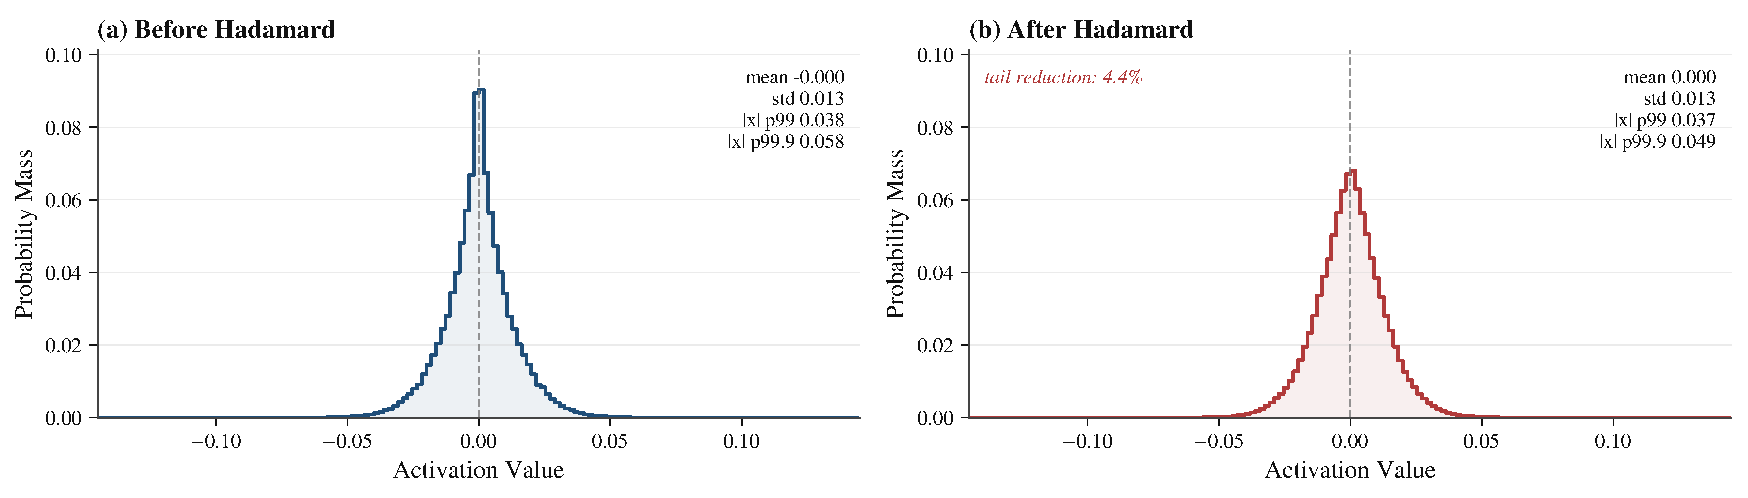
\includegraphics[width=0.86\textwidth]{figures/hadamard_activation_cropped.pdf}
\caption{Key-state activation distribution before and after Hadamard rotation on a Llama-2-7B sample. The rotation suppresses heavy tails while preserving enough variation for feature-level sparsification.}
\label{fig:hadamard}
\end{figure}

\begin{table}[tbp]
    \centering
    \small
    \caption{PPL of RTN and Hadamard rotation (\textit{Rotate}) on WikiText-2 under quantization-only and sparse-quant settings. Hadamard rotation improves low-bit quantization stability, while remaining compatible with subsequent KV sparsification.}
    \label{tab:hadamard_sparse_quant}
    \setlength{\tabcolsep}{4pt}
    \begin{tabular}{lcccccc}
        \toprule
        & \multicolumn{2}{c}{4-bit} & \multicolumn{2}{c}{3-bit} & \multicolumn{2}{c}{2-bit} \\
        \cmidrule(lr){2-3}
        \cmidrule(lr){4-5}
        \cmidrule(lr){6-7}
        Setting & RTN & Rotate & RTN & Rotate & RTN & Rotate \\
        \midrule
        Quant only
        & 5.22 & \textbf{5.14}
        & 6.57 & \textbf{5.28}
        & 115.55 & \textbf{5.35} \\
        +50\% KV sparsity
        & \textbf{5.27} & 5.69
        & 6.57 & \textbf{6.35}
        & 115.55 & \textbf{6.65} \\
        \bottomrule
    \end{tabular}
\end{table}

The remaining nonzero KV states still require a low-bit representation. We therefore adopt \emph{Per-Token-Tile} quantization, which aligns the quantization unit with token-level compression decisions and the tile-based decode path while providing a fine-grained low-bit representation.

For a token vector $\mathbf{x}_t \in \mathbb{R}^d$ (either key or value), the feature dimension is partitioned into $M=d/g$ contiguous tiles of size $g$:
\begin{equation}
\mathbf{x}_t = [\mathbf{x}_{t,1},\mathbf{x}_{t,2},\ldots,\mathbf{x}_{t,M}], \qquad \mathbf{x}_{t,m} \in \mathbb{R}^{g}.
\end{equation}
Each tile is quantized independently with its own scale $s_{t,m}$ and zero point $z_{t,m}$:
\begin{equation}
\mathbf{q}_{t,m}
=
\operatorname{clip}\!\left(
\operatorname{round}\!\left(
\frac{\mathbf{x}_{t,m}-z_{t,m}}{s_{t,m}}
\right),
0,\,
2^b-1
\right),
\end{equation}
where $b$ is the quantization bitwidth.

Since key states may contain outliers that destabilize aggressive low-bit quantization, \method\ applies Hadamard rotation to queries and keys before quantization. Let $\mathbf{H} \in \mathbb{R}^{d \times d}$ denote the normalized Hadamard matrix. We rotate

\begin{equation}
\tilde{\mathbf{q}}_i = \frac{1}{\sqrt{d}}\mathbf{H}\mathbf{q}_i,
\qquad
\tilde{\mathbf{k}}_j = \frac{1}{\sqrt{d}}\mathbf{H}\mathbf{k}_j.
\end{equation}
Because the Hadamard matrix is orthogonal, the attention score is preserved:
\begin{equation}
\tilde{\mathbf{q}}_i^\top \tilde{\mathbf{k}}_j
=
\mathbf{q}_i^\top \mathbf{k}_j.
\end{equation}

Figure~\ref{fig:hadamard} and Table~\ref{tab:hadamard_sparse_quant} show that Hadamard rotation suppresses heavy tails and improves low-bit robustness, especially at lower bitwidths.

% The rotation therefore improves the distribution seen by the quantizer without changing the attention computation itself.

% Figure~\ref{fig:hadamard} illustrates the effect of the Hadamard rotation on key states. After rotation, the heavy tail is noticeably suppressed, which reduces the dominance of outliers in low-bit quantization. At the same time, the rotated distribution does not collapse into a fully uniform one, and still preserves sufficient magnitude variation for subsequent magnitude-based feature sparsification.

% Table~\ref{tab:hadamard_sparse_quant} further supports this observation quantitatively on WikiText-2. Under quantization-only settings, Hadamard rotation improves PPL at 4-bit, 3-bit, and especially 2-bit, supporting its role in stabilizing low-bit quantization. When 50\% KV sparsity is further applied, the same trend remains visible at 3-bit and 2-bit, where Rotate still outperforms RTN by a meaningful margin. At 4-bit with added sparsity, however, the gain becomes marginal and slightly reverses, suggesting that when quantization error is already relatively small, the rotation-induced mixing may mildly weaken the magnitude separability used by subsequent sparsification. Overall, Per-Token-Tile quantization provides a fine-grained low-bit representation, while Hadamard rotation appears to improve robustness to key outliers without largely disrupting subsequent sparsification.


\subsection{Sparse-Quant Format and Decode Kernel}
\label{sec:sparse-quant}
\begin{figure}[t]
\centering
\begin{minipage}[t]{0.47\textwidth}
\centering
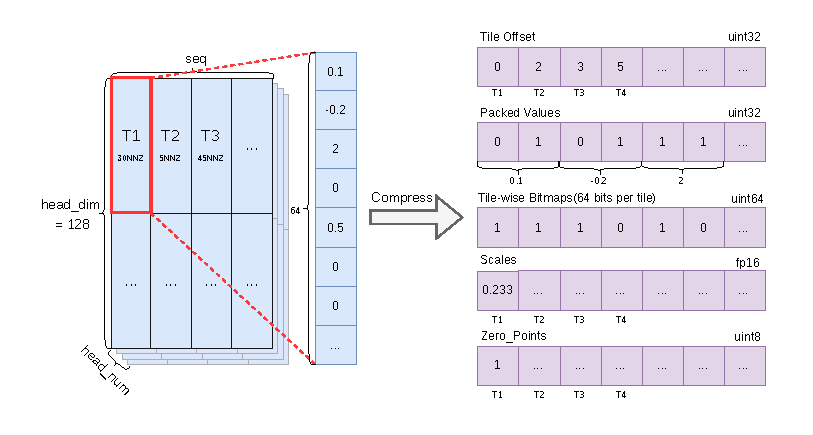
\includegraphics[width=0.98\linewidth]{figures/bitmap_sparse_quant_format.pdf}
\vspace{1mm}

\small (a) bitmap-based sparse-quant format
\end{minipage}\hfill
\begin{minipage}[t]{0.47\textwidth}
\centering
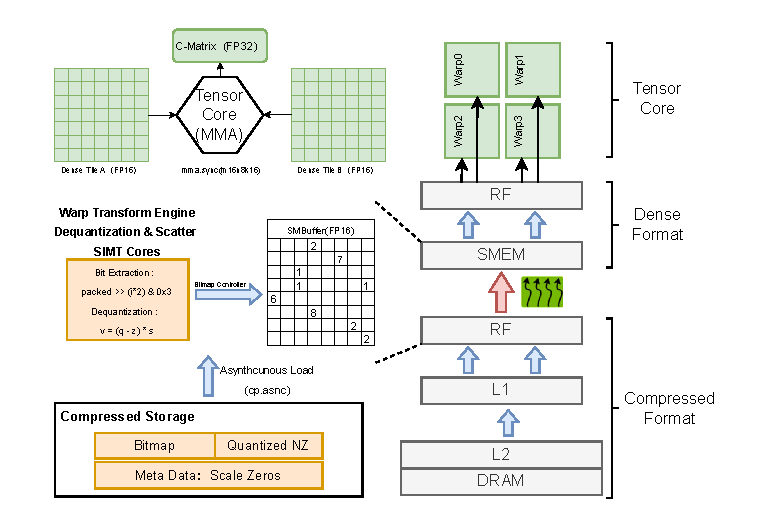
\includegraphics[width=0.98\linewidth]{figures/bitmap_sparse_quant_operator.pdf}
\vspace{1mm}

\small (b) Sparse-quant decode kernel
\end{minipage}
\caption{Sparse-quant format and decode kernel. The format stores bitmap metadata and packed low-bit values, while the kernel follows a load-as-compressed, compute-as-dense execution path.}
\label{fig:sq-kernel-overview}
\end{figure}

We co-design a sparse-quant format and a matching decode kernel so that compressed KV-cache representations reduce not only storage cost but also decode-time memory traffic.

Figure~\ref{fig:sq-kernel-overview} summarizes this design. Each $1 \times 64$ tile stores a bitmap for nonzero positions, packed low-bit values, a per-tile offset, and quantization metadata such as scales and zero points. During decode, the kernel follows a \emph{load-as-compressed, compute-as-dense} strategy: it loads compressed tiles from memory, reconstructs dense shared-memory tiles through unpacking and dequantization, and then invokes Tensor Core matrix-vector computation. In this way, sparsity is handled along the loading path while the compute stage remains dense and regular.

This design is particularly useful for decode-stage attention, which is strongly memory-bound: keeping the KV cache compressed in memory reduces memory traffic, while reconstructing dense tiles only on the compute path avoids irregular accesses and control-flow divergence.

% Figure~\ref{fig:sq-kernel-overview} gives an overview of this design. The left panel shows the sparse-quant format. Each $1 \times 64$ tile stores a bitmap for nonzero positions, packed low-bit values, a per-tile offset, and quantization metadata such as scales and zero points. This layout is designed to support high sparsity and low-bit storage while preserving a regular memory organization, thereby avoiding the irregular accesses and indexing overheads of conventional sparse formats.

% The right panel shows the matching decode kernel. During decode, the kernel follows a \emph{load-as-compressed, compute-as-dense} strategy. It first loads bitmaps and packed low-bit values from memory, then reconstructs the nonzeros through unpacking and dequantization, and scatters them into dense shared-memory tiles. Tensor Core matrix-vector computation is then performed on these reconstructed dense tiles. In this way, sparsity is handled only along the data-loading path, while the actual compute stage still uses regular dense operators.

% This design is particularly important for decode-stage attention, which is strongly memory-bound. By keeping the KV cache compressed in memory, the format reduces memory traffic; by reconstructing dense tiles only along the compute path, the kernel avoids the control-flow divergence and irregular accesses that often limit sparse execution. As a result, the sparse-quant format and decode kernel together convert compressed KV representations into practical decode-time gains, rather than merely reducing storage footprint.


\section{Experiments}
\label{sec:experiments}

\subsection{Experimental Setup}
Our implementation uses Python 3.10, PyTorch 2.6.0, CUDA 12.4, and custom CUDA/Triton kernels. All experiments are conducted on a single NVIDIA A100 80GB PCIe GPU with an Intel Xeon CPU and 252GB host memory.

For accuracy, we use the official LongBench~\cite{longbench} pipeline on six representative tasks: NarrativeQA, Qasper, \multifieldqa, HotpotQA, TREC, and LCC. We use Llama-3-8B-Instruct~\cite{grattafiori2024llama3} as the main model and additionally test Llama-2-7B~\cite{touvron2023llama2}, Mistral-7B-v0.1~\cite{jiang2023mistral7b}, and Qwen2.5-7B-Instruct~\cite{yang2024qwen25}. Inputs are truncated to 8192 tokens via head-tail truncation when needed. We compare against dense decoding, a matched-budget uniform sparsity baseline based on MUSTAFAR~\cite{joo2025mustafar}, and a sequential MUSTAFAR+KIVI baseline~\cite{liu2024kivi} (denoted as \textbf{M+K}). Sparse-only settings use 50\% and 70\% average sparsity, while joint sparse-quant settings use 50/50 and 70/70 K/V sparsity with 4-bit and 2-bit quantization. Differential policies are selected on a small calibration split and re-checked on a disjoint validation split before final evaluation on these tasks.

For efficiency, we use Llama-3-8B-Instruct with 4096 input tokens, 256 generated tokens, and batch sizes from 1 to 8, and report end-to-end throughput, compression overhead, compressed KV-cache size, and compression ratio. We compare dense decoding, the MUSTAFAR~\cite{joo2025mustafar} sparse kernel, and the proposed sparse-quant runtime path.

% For accuracy evaluation, we use LongBench~\cite{longbench} with the official pipeline. Our main sparse-only and joint sparse-quant comparisons focus on six focal tasks from this benchmark. These tasks are NarrativeQA, Qasper, \multifieldqa, HotpotQA, TREC, and LCC. They cover diverse long-context behaviors while enabling stable matched-budget comparisons across compression settings and model families. We use Llama-3-8B-Instruct~\cite{grattafiori2024llama3} as the main model and further evaluate on Llama-2-7B~\cite{touvron2023llama2}, Mistral-7B-v0.1~\cite{jiang2023mistral7b}, and Qwen2.5-7B-Instruct~\cite{yang2024qwen25}. Inputs are truncated to 8192 tokens by keeping the first 4096 and the last 4096 tokens when necessary. We compare against dense decoding, a uniform sparsity baseline using the MUSTAFAR sparsity setting~\cite{joo2025mustafar}, and a sequential sparse-then-quantize baseline that combines that sparsity setting with KIVI quantization~\cite{liu2024kivi}, denoted as \textbf{M+K}. We report 50\% and 70\% average sparsity for sparse-only comparisons, and 50/50 and 70/70 K/V sparsity with 4-bit and 2-bit quantization for joint sparse-quant comparisons. Differential policies are selected by a lightweight held-out calibration procedure; detailed reporting rules and finalized configurations are provided in Appendix~\ref{app:diffsparse-extra}.

\subsection{Accuracy Results}

\subsubsection{Differential Sparsity Alone}
\label{sec:diff-sparsity-alone}
We first study differential sparsity without quantization or Hadamard rotation to isolate the effect of budget allocation, comparing \method\ against dense decoding and a matched-budget uniform sparsity baseline at 50\% and 70\% average sparsity. Table~\ref{tab:diff-sparsity-meta-main} shows that differential sparsity remains non-negative and yields larger gains at 70\% sparsity than at 50\%, suggesting that token-level budget allocation becomes more valuable under tighter sparsity budgets.
\begin{table}[tbp]
\centering
\caption{Sparse-only results on six representative LongBench tasks for Llama-3-8B-Instruct.}
\label{tab:diff-sparsity-meta-main}
% \caption{Sparse-only differential sparsity versus matched-budget uniform sparsity on Llama-3-8B-Instruct over six representative LongBench tasks. Dense decoding is reported as an uncompressed reference. ``Uniform'' corresponds to the token-agnostic policy used in MUSTAFAR. In a few cases, the reported differential result reverts to the uniform baseline.}
\setlength{\tabcolsep}{4pt}
\resizebox{\textwidth}{!}{
\begin{tabular}{lccccccc}
\toprule
Method & NarrativeQA & Qasper & \multifieldqaheader & HotpotQA & TREC & LCC & Avg. \\
\midrule
Dense & 23.45 & 42.18 & 43.14 & 46.06 & 74.00 & 57.12 & 47.66 \\
\midrule
Uniform-50 & 23.44 & 43.73 & 42.93 & 45.94 & 73.50 & 56.03 & 47.59 \\
Differential-50 & 23.44 & 43.73 & 42.93 & 45.94 & \textbf{74.00} & \textbf{57.08} & \textbf{47.85} \\
\midrule
Uniform-70 & 23.94 & 40.89 & 40.91 & 44.93 & 70.00 & 54.12 & 45.80 \\
Differential-70 & 23.94 & \textbf{41.03} & \textbf{41.61} & \textbf{45.12} & \textbf{72.50} & \textbf{55.45} & \textbf{46.61} \\
\bottomrule
\end{tabular}}
\end{table}



% \begin{table}[t]
% \centering
% \caption{Cross-model average sparse-only results on six representative LongBench tasks.}
% \caption{Cross-model average sparse-only results on six representative LongBench tasks under matched sparsity budgets.}
% \caption{Cross-model average sparse-only results on the six representative LongBench tasks. ``Differential'' denotes the finalized full-task average under the same reporting protocol as the main-text sparse-only study.}
% \label{tab:diff-sparsity-cross-model-main}
% \setlength{\tabcolsep}{5pt}
% \resizebox{0.82\textwidth}{!}{
% \begin{tabular}{lcccc}
% \toprule
% Model & Budget & Uniform Avg. & Differential Avg. & $\Delta$ \\
% \midrule
% Llama-2-7B & 50\% & 30.88 & \textbf{31.54} & +0.66 \\
% Llama-2-7B & 70\% & 29.29 & \textbf{30.78} & +1.49 \\
% Qwen2.5-7B-Instruct & 50\% & 31.56 & \textbf{31.68} & +0.11 \\
% Qwen2.5-7B-Instruct & 70\% & 30.67 & \textbf{31.24} & +0.57 \\
% \bottomrule
% \end{tabular}}
% \end{table}

% \begin{table}[tbp]
% \centering
% \caption{Cross-model sparse-only averages on six representative LongBench tasks.}
% \label{tab:diff-sparsity-cross-model-main}
% \setlength{\tabcolsep}{5pt}
% \resizebox{0.78\textwidth}{!}{
% \begin{tabular}{lcccc}
% \toprule
% Model & Budget & Uniform & Differential & $\Delta$ \\
% \midrule
% \multirow{2}{*}{Llama-2-7B}
% & 50\% & 30.88 & \textbf{31.54} & +0.66 \\
% & 70\% & 29.29 & \textbf{30.78} & +1.49 \\
% \midrule
% \multirow{2}{*}{Qwen2.5-7B-Instruct}
% & 50\% & 31.56 & \textbf{31.68} & +0.11 \\
% & 70\% & 30.67 & \textbf{31.24} & +0.57 \\
% \bottomrule
% \end{tabular}}
% \end{table}

% The same trend holds across models: differential sparsity stays non-negative and yields larger gains at 70\% sparsity than at 50\% (Table~\ref{tab:diff-sparsity-cross-model-main}). Together, Tables~\ref{tab:diff-sparsity-meta-main} and~\ref{tab:diff-sparsity-cross-model-main} show that token-level budget allocation is already beneficial in the sparse-only regime and becomes more important under tighter budgets.

\subsubsection{Joint Sparsity-Quantization Results}

\begin{table}[tbp]
\centering
\caption{Joint sparse-quant results on six representative LongBench tasks for Llama-3-8B-Instruct.}
\label{tab:main-accuracy}
\setlength{\tabcolsep}{4pt}
\resizebox{\textwidth}{!}{
\begin{tabular}{lccccccc}
\toprule
Setting & NarrativeQA & Qasper & \multifieldqaheader & HotpotQA & TREC & LCC & Avg. \\
\midrule
M+K, 50/50 + 4-bit & 21.61 & \textbf{40.70} & \textbf{47.62} & 41.13 & \textbf{70.50} & 53.83 & 45.90 \\
\method, 50/50 + 4-bit & \textbf{21.92} & 39.38 & 46.77 & \textbf{41.38} & \textbf{70.50} & \textbf{55.64} & \textbf{45.93} \\
M+K, 50/50 + 2-bit & \textbf{21.97} & 38.96 & \textbf{46.11} & 40.39 & 68.00 & 44.86 & 43.38 \\
\method, 50/50 + 2-bit & 21.16 & \textbf{39.54} & 44.49 & \textbf{41.19} & \textbf{71.50} & \textbf{46.26} & \textbf{44.02} \\
M+K, 70/70 + 4-bit & 20.94 & 37.32 & 44.90 & \textbf{41.22} & 68.00 & 52.71 & 44.18 \\
\method, 70/70 + 4-bit & \textbf{21.86} & \textbf{38.81} & \textbf{46.52} & 40.64 & \textbf{70.00} & \textbf{54.23} & \textbf{45.34} \\
M+K, 70/70 + 2-bit & \textbf{21.34} & 35.43 & 43.43 & 39.21 & 63.00 & 36.59 & 39.83 \\
\method, 70/70 + 2-bit & 19.70 & \textbf{39.49} & \textbf{44.31} & \textbf{40.15} & \textbf{70.00} & \textbf{45.04} & \textbf{43.12} \\
\bottomrule
\end{tabular}}
\end{table}

Table~\ref{tab:main-accuracy} reports joint sparse-quant results on six representative LongBench tasks for Llama-3-8B-Instruct~\cite{grattafiori2024llama3}. Across all four settings, \method\ achieves higher average scores than the sequential M+K baseline, with the largest gain at 70/70 + 2-bit, where the average score improves from 39.83 to 43.12. This supports jointly aligning sparsity, quantization, and runtime execution under tighter compression budgets. A quantization-only comparison isolating the contribution of the proposed low-bit representation is reported in \ref{app:quant-only}.

\begin{table}[tbp]
\centering
\caption{Cross-model joint sparse-quant averages on six representative LongBench tasks.}
\label{tab:cross-model}
\scriptsize
\renewcommand{\arraystretch}{0.94}
\setlength{\tabcolsep}{2.5pt}
\resizebox{\textwidth}{!}{
\begin{tabular}{lcccccccc}
\toprule
& \multicolumn{2}{c}{50/50 + 4-bit}
& \multicolumn{2}{c}{50/50 + 2-bit}
& \multicolumn{2}{c}{70/70 + 4-bit}
& \multicolumn{2}{c}{70/70 + 2-bit} \\
\cmidrule(lr){2-3}
\cmidrule(lr){4-5}
\cmidrule(lr){6-7}
\cmidrule(lr){8-9}
Model & M+K & \method & M+K & \method & M+K & \method & M+K & \method \\
\midrule
Llama-2-7B & 31.34 & \textbf{31.37} & \textbf{31.51} & 30.23 & 30.57 & \textbf{30.97} & 29.92 & \textbf{30.09} \\
Mistral-7B-v0.1 & 32.84 & \textbf{32.90} & 31.70 & \textbf{32.37} & 32.43 & \textbf{32.71} & 30.14 & \textbf{32.35} \\
Qwen2.5-7B-Instruct & 31.17 & \textbf{37.08} & \textbf{26.10} & 23.48 & 33.00 & \textbf{39.67} & 25.51 & \textbf{35.20} \\
\bottomrule
\end{tabular}
}
\end{table}

Table~\ref{tab:cross-model} shows a generally favorable but non-uniform cross-model trend over M+K: gains are more consistent under tighter compression budgets, while a few milder settings remain neutral or slightly negative. This suggests that the benefit of \method\ mainly comes from the joint design itself, although its magnitude still depends on model family and compression setting.

\subsection{Efficiency Results}
In efficiency experiments, we compare \method\ against dense decoding and the executable MUSTAFAR sparse kernel~\cite{joo2025mustafar}, since the sequential \textbf{M+K} baseline does not provide a unified end-to-end runtime path.
\subsubsection{End-to-End Throughput}

% \begin{table}[!t]
% \centering
% \caption{End-to-end decoding throughput (tokens/s) on Llama-3-8B-Instruct with 4096 input tokens and 256 output tokens.}
% \label{tab:throughput-table}
% \setlength{\tabcolsep}{4pt}
% \resizebox{\textwidth}{!}{
% \begin{tabular}{cccccc}
% \toprule
% Batch Size & Dense & MUSTAFAR-50 & MUSTAFAR-70 & \method\ 50/50 + 2-bit & \method\ 70/70 + 2-bit \\
% \midrule
% 1 & 28.55 & 17.16 & 16.84 & 23.24 & 23.38 \\
% 2 & 39.81 & 31.75 & 30.56 & 42.76 & 42.37 \\
% 3 & 49.15 & 45.15 & 46.18 & 55.45 & 57.81 \\
% 4 & 55.83 & 53.80 & 57.63 & 64.70 & 66.42 \\
% 5 & 56.67 & 66.93 & 65.96 & 72.02 & 74.22 \\
% 6 & 56.81 & 77.17 & 78.01 & 76.80 & 80.38 \\
% 7 & 59.69 & 86.52 & 83.53 & 80.47 & 84.06 \\
% 8 & 62.80 & 94.51 & 96.43 & 86.98 & 87.12 \\
% \bottomrule
% \end{tabular}}
% \end{table}

\begin{wrapfigure}{r}{0.48\textwidth}
\centering
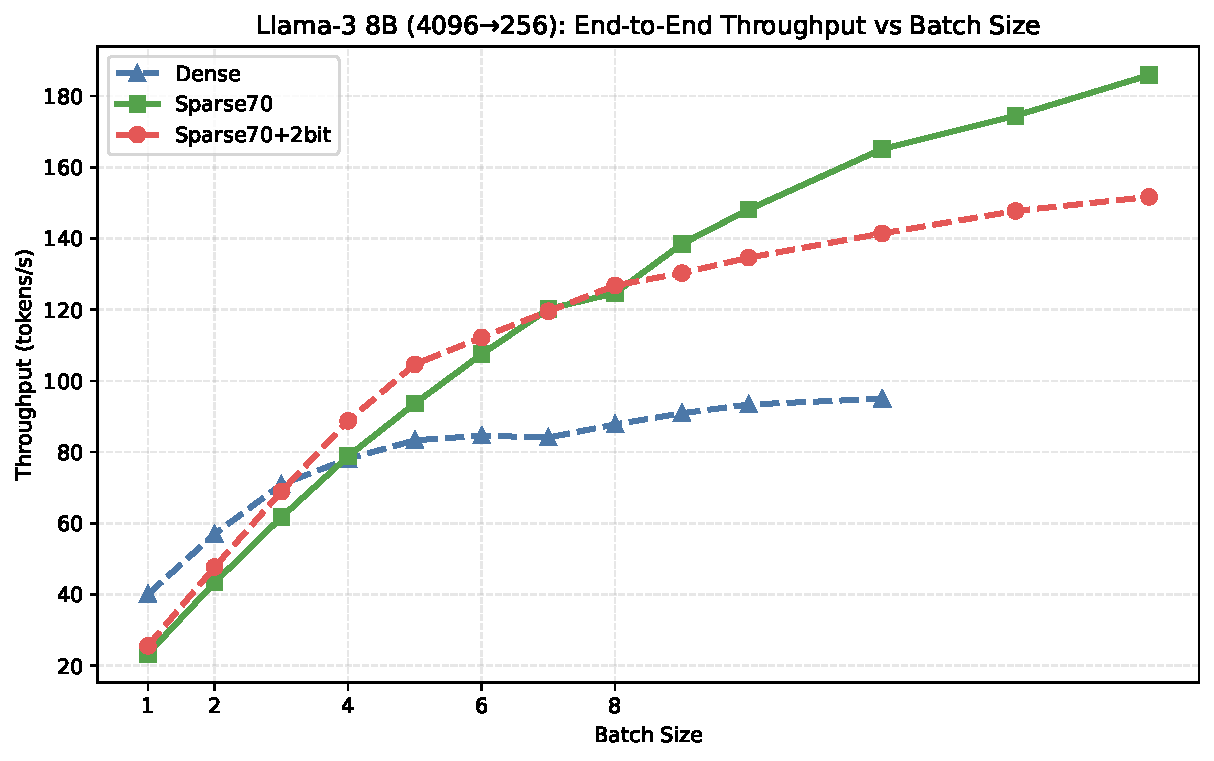
\includegraphics[width=0.46\textwidth]{figures/throughput_llama3_bs.pdf}
\caption{End-to-end decoding throughput on Llama-3-8B. The clearest gain appears in the small-to-medium batch regime.}
\label{fig:throughput}
\end{wrapfigure}

Figure~\ref{fig:throughput} reports end-to-end decoding throughput on Llama-3-8B-Instruct~\cite{grattafiori2024llama3}. Dense decoding is strongest at batch size 1, where compression overhead is not yet amortized. As batch size increases, the compressed paths become more favorable, with the clearest sparse-quant advantage in the small-to-medium batch regime. Under 70/70 + 2-bit, \method\ reaches 80.38 tokens/s at batch size 6, improving over dense decoding by 41.5\% and over MUSTAFAR-70 by 3.0\%. At larger batch sizes, the gap narrows, suggesting that unpacking and dequantization overheads are less effectively amortized once the workload becomes more compute-heavy.

% Table~\ref{tab:throughput-table} and Fig.~\ref{fig:throughput} report end-to-end decoding throughput on Llama-3-8B-Instruct~\cite{grattafiori2024llama3}. Dense decoding is strongest at batch size 1, where the compression overhead is not yet amortized. As batch size increases, the compressed paths become increasingly favorable, indicating that the workload becomes more bandwidth-sensitive. The most visible advantage of the full sparse-quant design appears in the small-to-medium batch regime. For example, under the 70/70 + 2-bit setting, \method\ reaches 80.38 tokens/s at batch size 6, which is 41.5\% higher than dense decoding and 3.0\% higher than MUSTAFAR-70. At larger batch sizes, however, the throughput gap narrows and sparsity-only configurations can become preferable, suggesting that the extra unpacking and dequantization overhead is less effectively amortized once the workload becomes more compute-heavy. Overall, these results suggest that joint sparse-quant compression can translate into practical decoding speedups when KV-cache traffic remains the dominant bottleneck.

\subsubsection{Compression Overhead}

% Compression is beneficial only when its own runtime cost remains controlled. Table~\ref{tab:compression-summary} reports representative compression statistics on Llama-3-8B-Instruct. The results show that the sparse-quant path achieves substantially higher compression ratios than sparsity-only baselines while keeping compression time competitive. For example, at batch size 8, MUSTAFAR-70 reduces the KV cache to 1964.29MB, whereas \method\ under the 70/70 + 2-bit setting further reduces it to 1176.25MB, improving the compression ratio from 2.09$\times$ to 3.48$\times$, while also lowering compression time from 5411.29ms to 4293.18ms. This suggests that the benefit of \method\ is not limited to reduced decode-time bandwidth demand; the more compact sparse-quant representation also reduces compression-side write-back cost.

\begin{table}[tbp]
\centering
\scriptsize
\renewcommand{\arraystretch}{0.94}
\caption{Compression statistics at input length 4096.}
\label{tab:compression-summary}
\setlength{\tabcolsep}{3.2pt}
\begin{tabular*}{0.96\textwidth}{@{\extracolsep{\fill}}lcccccc@{}}
\toprule
& \multicolumn{3}{c}{BS = 1} & \multicolumn{3}{c}{BS = 8} \\
\cmidrule(lr){2-4}\cmidrule(lr){5-7}
Method & KV (MB) & Ratio & Time (ms) & KV (MB) & Ratio & Time (ms) \\
\midrule
Sparse-50 & 2720.2 & 1.51$\times$ & 740.8 & 2720.2 & 1.51$\times$ & 5688.2 \\
Sparse-70 & 1964.3 & 2.09$\times$ & 716.3 & 1964.3 & 2.09$\times$ & 5411.3 \\
Sparse-50 + 2b & 1261.2 & 3.25$\times$ & 545.2 & 1261.2 & 3.25$\times$ & 4317.9 \\
Sparse-70 + 2b & 1176.3 & 3.48$\times$ & 552.9 & 1176.3 & 3.48$\times$ & 4293.2 \\
\bottomrule
\end{tabular*}
\end{table}

Table~\ref{tab:compression-summary} reports representative compression statistics on Llama-3-8B-Instruct. Compared with sparsity-only baselines, the sparse-quant path achieves higher compression ratios while keeping compression time competitive. At batch size 8, \method\ under 70/70 + 2-bit reduces the KV cache from 1964.3MB to 1176.3MB relative to MUSTAFAR-70, improving the compression ratio from 2.09$\times$ to 3.48$\times$ and reducing compression time from 5411.3ms to 4293.2ms. This suggests that the more compact sparse-quant representation also lowers compression-side write-back cost.

% \section{Discussion and Future Work}
% \label{sec:discussion}

% Although JSQKV achieves a favorable trade-off between accuracy and efficiency in long-context settings, several limitations remain for future work.

% First, the current method relies on explicit token-importance estimation rather than a uniform sparsity budget, but this modeling still mainly operates at the token level. It does not yet capture finer-grained sensitivity across layers, attention heads, or Key/Value representations. A more fine-grained joint design of importance modeling and quantization is therefore worth exploring.

% Second, the joint sparse-quant path is not advantageous under all serving conditions. Its largest throughput gains appear in small- to medium-batch scenarios, whereas at larger batch sizes the benefit of compression is increasingly offset by dequantization, metadata handling, and higher compute pressure. Designing more efficient sparse-quant operators thus remains an important direction.

% Finally, the current evaluation scope is still limited. Although the experiments cover multiple model families and representative long-context settings, further study is needed to verify whether the proposed method remains effective in ultra-long-context scenarios, on heterogeneous accelerators, and in production-like deployment environments.

\section{Conclusion}
\label{sec:conclusion}

\method\ reduces KV-cache cost through differential sparsification, stabilized low-bit quantization, and a bitmap-based sparse-quant decode kernel. Evaluation results show that, under matched compression budgets, \method\ generally compares favorably with a sequential sparsity-plus-quantization baseline, with larger gains under more aggressive sparse-quant settings. These results further show that compression savings can translate into practical throughput gains during decoding. Overall, these findings support treating KV-cache compression as a systems-and-algorithms co-design problem rather than as a simple composition of independent post-processing steps.



% \clearpage
\appendix
\setcounter{section}{0}
\renewcommand{\thesection}{Appendix \arabic{section}}

%%% 以下是附录缩减版
\section{Threshold Stability for Prefill-to-Decode Reuse}
\label{sec:appendix-threshold-reuse}

Section~\ref{sec:diff-sparsity} estimates the token-importance thresholds
$(\tau_{\text{high}}, \tau_{\text{low}})$ from normalized prefill attention,
and Section~\ref{sec:dual-window} reuses the same thresholds during decoding
after normalizing the accumulated attention by the number of available future
observations. This reuse strategy relies on a simple layer-wise stability
assumption: under the same normalization rule, the importance-score scale of a
fixed layer should remain sufficiently consistent for prefill-estimated
thresholds to remain meaningful during online decoding.

We test this assumption using the same threshold definition as \method. We
compute normalized attention-derived importance scores from the observed
attention statistics and derive the corresponding thresholds
$(\tau_{\text{high}}, \tau_{\text{low}})$. The evaluation is conducted on
Llama-3-8B-Instruct~\cite{grattafiori2024llama3} using seven datasets:
WikiText-2~\cite{merity2016pointer}, GSM8K~\cite{cobbe2021gsm8k},
MuSiQue~\cite{trivedi2022musique}, and four LongBench tasks: Qasper,
\multifieldqa, NarrativeQA, and HotpotQA~\cite{longbench}. Each dataset
contributes 10 samples, and we evaluate layers 10 and 20 as representative
layers.

Table~\ref{tab:appendix-threshold-reuse} reports the resulting cross-dataset
statistics. For Layer 10, the median CV is 10.21\% for
$\tau_{\text{high}}$ and 14.37\% for $\tau_{\text{low}}$; for Layer 20, the
corresponding values are 19.40\% and 19.82\%. Figure~\ref{fig:appendix-threshold-reuse}
shows the full distributions. Two observations matter most. First, for a fixed
layer, both thresholds remain concentrated within a bounded range across
datasets. Second, the threshold scale is clearly layer dependent, so the
supported claim is reuse of \emph{fixed per-layer thresholds}, not a single
global threshold shared by all layers.

These results are sufficient for the reuse mechanism in
Section~\ref{sec:dual-window}. The decoder does not require decode-time scores
to match prefill thresholds exactly for every sample; it only requires the
normalized scores to stay on a comparable layer-wise scale. Taken together,
Table~\ref{tab:appendix-threshold-reuse} and
Figure~\ref{fig:appendix-threshold-reuse} support estimating
$(\tau_{\text{high}}, \tau_{\text{low}})$ once in prefill and reusing them
during decoding without step-wise re-calibration.

\begin{table}[t]
\centering
\caption{Cross-dataset stability of the normalized attention thresholds used by
the prefill-to-decode reuse path. CV is computed from the per-dataset median
thresholds.}
\label{tab:appendix-threshold-reuse}
\small
\begin{tabular}{llcc}
\toprule
Layer & Threshold & Median range & Median CV (\%) \\
\midrule
10 & $\tau_{\text{high}}$ & 0.67120--0.92427 & 10.21 \\
10 & $\tau_{\text{low}}$  & 0.04243--0.06552 & 14.37 \\
20 & $\tau_{\text{high}}$ & 0.35568--0.61690 & 19.40 \\
20 & $\tau_{\text{low}}$  & 0.01732--0.02890 & 19.82 \\
\bottomrule
\end{tabular}
\end{table}

\begin{figure}[t]
\centering
\begin{minipage}[t]{0.47\linewidth}
\centering

\includegraphics[width=\linewidth]{\attnscorefigdir/layer10_normalized_attention_thresholds.pdf}
\end{minipage}\hfill
\begin{minipage}[t]{0.47\linewidth}
\centering

\includegraphics[width=\linewidth]{\attnscorefigdir/layer20_normalized_attention_thresholds.pdf}
\end{minipage}
\caption{Cross-dataset distributions of the normalized attention thresholds
used by the prefill-to-decode reuse path. Left: Layer 10. Right: Layer 20. The
thresholds remain stable at a fixed layer, while their absolute scale is
layer dependent.}
\label{fig:appendix-threshold-reuse}
\end{figure}

\FloatBarrier
\section{Additional Quantization-Only Comparison}
\label{app:quant-only}

To isolate the contribution of the numerical representation in \method, we compare a quantization-only instantiation of the \method\ quantizer against a matched KIVI baseline~\cite{liu2024kivi}. This appendix keeps the same per-token-tile low-bit representation used by \method\ but removes differential sparsity and the bitmap-based sparse runtime path.

Unless otherwise noted, both methods use a residual window of 128 tokens. The KIVI baseline uses channel-wise key quantization, per-token-head value quantization, and group size 128, whereas the \method\ quantizer uses per-token-tile quantization with tile-wise Hadamard rotation (tile size 64 and Hadamard group size 64).

Table~\ref{tab:appendix-quant-llama3} reports quantization-only results on representative LongBench tasks for Llama-3-8B-Instruct~\cite{grattafiori2024llama3}. At 4-bit and 3-bit, the two methods remain close in average score. At 2-bit, however, the \method\ quantizer is noticeably stronger, improving the average over the representative tasks from 25.83 to 28.39, with especially visible gains on HotpotQA and LCC. This pattern suggests that the tile-aligned design is most helpful in the aggressive low-bit regime.

Table~\ref{tab:appendix-quant-crossmodel} summarizes the same comparison on additional model families using representative LongBench tasks. It is intended to show whether the quantization trend transfers under comparable representative-task settings, rather than to support strict cross-row ranking under an identical task set. The \method\ quantizer remains competitive on Llama-2-7B and becomes favorable at 2-bit on Mistral-7B-v0.1, suggesting that its main benefit is improved robustness under aggressive low-bit quantization.

\begin{table}[t]
\centering
\caption{Quantization-only comparison on representative LongBench tasks for Llama-3-8B-Instruct. Avg.\ is computed over the reported representative tasks.}
\label{tab:appendix-quant-llama3}
\setlength{\tabcolsep}{4pt}
\resizebox{\textwidth}{!}{
\begin{tabular}{lcccccccc}
\toprule
Setting & Bit & NarrativeQA & HotpotQA & GovReport & TREC & PCount & LCC & Avg. \\
\midrule
KIVI & 4-bit & \textbf{24.26} & 46.06 & 29.53 & \textbf{74.00} & \textbf{6.50} & 54.07 & 39.07 \\
\method\ quantizer & 4-bit & 22.47 & \textbf{46.07} & \textbf{30.03} & 73.50 & 5.50 & \textbf{57.20} & \textbf{39.13} \\
KIVI & 3-bit & 20.81 & 45.64 & \textbf{29.35} & \textbf{74.00} & 6.75 & \textbf{60.94} & \textbf{39.58} \\
\method\ quantizer & 3-bit & \textbf{21.64} & \textbf{46.62} & 29.16 & 73.50 & \textbf{7.00} & 53.66 & 38.60 \\
KIVI & 2-bit & 16.55 & 27.50 & 23.91 & \textbf{58.00} & 2.00 & 27.03 & 25.83 \\
\method\ quantizer & 2-bit & \textbf{17.90} & \textbf{37.93} & \textbf{25.63} & 55.50 & \textbf{3.00} & \textbf{30.37} & \textbf{28.39} \\
\bottomrule
\end{tabular}}
\end{table}

\begin{table}[t]
\centering
\caption{Cross-model quantization-only averages on representative LongBench tasks. $\Delta$ is ``\method\ quantizer minus KIVI''.}
\label{tab:appendix-quant-crossmodel}
\setlength{\tabcolsep}{3.5pt}
\resizebox{\textwidth}{!}{
\begin{tabular}{lcccccccccc}
\toprule
Model & Protocol & KIVI 4-bit & \method\ 4-bit & $\Delta$ & KIVI 3-bit & \method\ 3-bit & $\Delta$ & KIVI 2-bit & \method\ 2-bit & $\Delta$ \\
\midrule
Llama-3-8B-Instruct & representative LongBench tasks & 39.07 & \textbf{39.13} & \textbf{+0.06} & \textbf{39.58} & 38.60 & -0.98 & 25.83 & \textbf{28.39} & \textbf{+2.56} \\
Llama-2-7B & representative LongBench tasks & 28.09 & \textbf{28.33} & \textbf{+0.24} & \textbf{28.23} & 27.82 & -0.41 & \textbf{24.33} & 24.17 & -0.16 \\
Mistral-7B-v0.1 & representative LongBench tasks & \textbf{31.19} & 30.78 & -0.41 & \textbf{30.16} & 29.52 & -0.64 & 23.91 & \textbf{25.72} & \textbf{+1.81} \\
\bottomrule
\end{tabular}}
\end{table}

\FloatBarrier
% \section{Additional Sparse-Only Reporting Details}
% \label{app:diffsparse-extra}

% This appendix provides additional details for the sparse-only differential-sparsity study, including task-level results for the additional models and the corresponding finalized retained configurations. These materials are omitted from the main text for space reasons. As in the main text, all sparse-only results follow the same conservative reporting protocol: candidate differential policies are selected on a small calibration split, re-checked on a disjoint validation split, and reverted to the matched-budget uniform baseline when the differential policy does not yield a stable gain on the final full-task evaluation.
% \subsection{Task-Level Sparse-Only Results for Additional Models}
% \label{app:diffsparse-tasklevel}

% Table~\ref{tab:appendix-diffsparse-llama7b}, Table~\ref{tab:appendix-diffsparse-qwen}, Table~\ref{tab:appendix-diffsparse-mistral}, and Table~\ref{tab:appendix-diffsparse-llama13b-70} report finalized sparse-only task-level results for the additional models summarized in the main text. As in the main sparse-only study, ``Differential'' denotes the finalized reported result after applying the same conservative reporting protocol.

% \begin{table}[t]
% \centering
% \caption{Task-level sparse-only results on Llama-2-7B~\cite{touvron2023llama2} over six representative LongBench tasks.}
% \label{tab:appendix-diffsparse-llama7b}
% \setlength{\tabcolsep}{4pt}
% \resizebox{\textwidth}{!}{
% \begin{tabular}{lccccccc}
% \toprule
% Method & NarrativeQA & Qasper & \multifieldqaheader & HotpotQA & TREC & LCC & Avg. \\
% \midrule
% Uniform-50 & 15.04 & 9.05 & 20.90 & 7.39 & 66.00 & 66.88 & 30.88 \\
% Differential-50 & 16.94 & 9.05 & 22.92 & 7.39 & 66.00 & 66.91 & 31.54 \\
% \midrule
% Uniform-70 & 13.66 & 7.69 & 19.42 & 6.57 & 64.50 & 63.89 & 29.29 \\
% Differential-70 & 15.00 & 7.88 & 22.73 & 6.96 & 65.50 & 66.59 & 30.78 \\
% \bottomrule
% \end{tabular}}
% \end{table}

% \begin{table}[t]
% \centering
% \caption{Task-level sparse-only results on Qwen2.5-7B-Instruct~\cite{yang2024qwen25} over six representative LongBench tasks.}
% \label{tab:appendix-diffsparse-qwen}
% \setlength{\tabcolsep}{4pt}
% \resizebox{\textwidth}{!}{
% \begin{tabular}{lccccccc}
% \toprule
% Method & NarrativeQA & Qasper & \multifieldqaheader & HotpotQA & TREC & LCC & Avg. \\
% \midrule
% Uniform-50 & 9.73 & 11.62 & 29.88 & 9.03 & 69.50 & 59.63 & 31.56 \\
% Differential-50 & 9.73 & 12.05 & 29.88 & 9.03 & 69.50 & 59.86 & 31.68 \\
% \midrule
% Uniform-70 & 8.60 & 11.04 & 28.52 & 8.76 & 68.00 & 59.11 & 30.67 \\
% Differential-70 & 9.33 & 11.72 & 28.61 & 9.68 & 69.00 & 59.11 & 31.24 \\
% \bottomrule
% \end{tabular}}
% \end{table}

% \begin{table}[t]
% \centering
% \caption{Task-level sparse-only results on Mistral-7B-v0.1~\cite{jiang2023mistral7b} over six focal LongBench tasks.}
% \label{tab:appendix-diffsparse-mistral}
% \setlength{\tabcolsep}{4pt}
% \resizebox{\textwidth}{!}{
% \begin{tabular}{lccccccc}
% \toprule
% Method & NarrativeQA & Qasper & \multifieldqaheader & HotpotQA & TREC & LCC & Avg. \\
% \midrule
% Uniform-50 & 12.99 & 28.89 & 39.92 & 26.24 & 67.50 & 53.46 & 38.17 \\
% Differential-50 & 12.99 & 29.46 & 40.37 & 26.24 & 67.50 & 53.46 & 38.34 \\
% \midrule
% Uniform-70 & 13.38 & 26.64 & 38.83 & 26.67 & 66.50 & 53.44 & 37.58 \\
% Differential-70 & 13.38 & 26.98 & 40.65 & 26.67 & 67.00 & 53.44 & 38.02 \\
% \bottomrule
% \end{tabular}}
% \end{table}

% \begin{table}[t]
% \centering
% \caption{Task-level sparse-only results on Llama-2-13B~\cite{touvron2023llama2} over six focal LongBench tasks at 70\% sparsity.}
% \label{tab:appendix-diffsparse-llama13b-70}
% \setlength{\tabcolsep}{4pt}
% \resizebox{\textwidth}{!}{
% \begin{tabular}{lccccccc}
% \toprule
% Method & NarrativeQA & Qasper & \multifieldqaheader & HotpotQA & TREC & LCC & Avg. \\
% \midrule
% Uniform-70 & 7.03 & 5.62 & 13.52 & 13.91 & 51.00 & 57.59 & 24.78 \\
% Differential-70 & 11.19 & 6.97 & 17.46 & 13.91 & 70.00 & 65.11 & 30.77 \\
% \bottomrule
% \end{tabular}}
% \end{table}

% For Llama-2-13B~\cite{touvron2023llama2} at 50\% sparsity, most focal tasks do not yet have stable full-task follow-up results under the reporting protocol used in this paper. We therefore omit a task-level table for that setting and report only the finalized average-level summary where available.

% \subsubsection{Finalized Per-Task Reporting Decisions}
% \label{app:diffsparse-decisions}

% Table~\ref{tab:appendix-diffsparse-decision-summary} summarizes, for each retained model and sparsity budget, how many of the six focal LongBench tasks ultimately keep a differential policy and how many revert to the matched-budget uniform baseline. This summary is intended to clarify the reporting protocol without overloading the main text with task-level bookkeeping.

% \begin{table}[t]
% \centering
% \caption{Summary of finalized sparse-only reporting decisions on the six focal LongBench tasks. ``Differential retained'' counts tasks whose final reported full-task result uses a differential policy; ``Uniform revert'' counts tasks whose final reported result reverts to the matched-budget uniform baseline.}
% \label{tab:appendix-diffsparse-decision-summary}
% \setlength{\tabcolsep}{6pt}
% \resizebox{0.86\textwidth}{!}{
% \begin{tabular}{lccc}
% \toprule
% Model & Budget & Differential retained & Uniform revert \\
% \midrule
% Llama-3-8B-Instruct & 50\% & 2 / 6 & 4 / 6 \\
% Llama-3-8B-Instruct & 70\% & 5 / 6 & 1 / 6 \\
% Llama-2-7B & 50\% & 4 / 6 & 2 / 6 \\
% Llama-2-7B & 70\% & 6 / 6 & 0 / 6 \\
% Qwen2.5-7B-Instruct & 50\% & 3 / 6 & 2 / 6, 1 tie \\
% Qwen2.5-7B-Instruct & 70\% & 5 / 6 & 1 / 6 \\
% Mistral-7B-v0.1 & 50\% & 2 / 6 & 4 / 6 \\
% Mistral-7B-v0.1 & 70\% & 3 / 6 & 3 / 6 \\
% Llama-2-13B & 70\% & 5 / 6 & 1 / 6 \\
% \bottomrule
% \end{tabular}}
% \end{table}

% \FloatBarrier
% \subsection{Finalized Retained Configurations}
% \label{app:diffsparse-configs}

% The tables below list the finalized retained configurations used in the sparse-only reporting. For readability, we report the target proportion distribution $[p_0,p_1,p_2]$, the corresponding sparsity levels $[\rho_0,\rho_1,\rho_2]$, and the final reporting decision for each task. Tasks marked as ``uniform revert'' use the matched-budget uniform baseline in the final reported result.

% \begin{table}[t]
% \centering
% \caption{Finalized sparse-only retained configurations for Llama-3-8B-Instruct~\cite{grattafiori2024llama3}.}
% \label{tab:appendix-meta-configs}
% \scriptsize
% \resizebox{\textwidth}{!}{
% \begin{tabular}{cccccc}
% \toprule
% Budget & Task & Final decision & $[p_0,p_1,p_2]$ & $[\rho_0,\rho_1,\rho_2]$ & Notes \\
% \midrule
% 50\% & narrativeqa & uniform revert & -- & -- & revert to matched-budget uniform \\
% 50\% & qasper & uniform revert & -- & -- & revert to matched-budget uniform \\
% 50\% & multifieldqa\_en & uniform revert & -- & -- & revert to matched-budget uniform \\
% 50\% & hotpotqa & uniform revert & -- & -- & revert to matched-budget uniform \\
% 50\% & trec & differential & $[0.0,0.833333,0.166667]$ & $[0.0,0.4,1.0]$ & value\_aware, max, sink=2 \\
% 50\% & lcc & differential & $[0.0,0.833333,0.166667]$ & $[0.0,0.4,1.0]$ & value\_aware, max, sink=2 \\
% \midrule
% 70\% & narrativeqa & uniform revert & -- & -- & revert to matched-budget uniform \\
% 70\% & qasper & differential & $[0.0,0.857143,0.142857]$ & $[0.0,0.65,1.0]$ & value\_aware, mean, sink=4 \\
% 70\% & multifieldqa\_en & differential & $[0.02,0.8,0.18]$ & $[0.0,0.65,1.0]$ & value\_aware, max, sink=4 \\
% 70\% & hotpotqa & differential & $[0.0,0.75,0.25]$ & $[0.0,0.6,1.0]$ & default settings \\
% 70\% & trec & differential & $[0.0,0.75,0.25]$ & $[0.0,0.6,1.0]$ & default settings \\
% 70\% & lcc & differential & $[0.0,0.75,0.25]$ & $[0.0,0.6,1.0]$ & default settings \\
% \bottomrule
% \end{tabular}}
% \end{table}

% \begin{table}[t]
% \centering
% \caption{Finalized sparse-only retained configurations for Llama-2-7B~\cite{touvron2023llama2}.}
% \label{tab:appendix-llama7b-configs}
% \scriptsize
% \resizebox{\textwidth}{!}{
% \begin{tabular}{cccccc}
% \toprule
% Budget & Task & Final decision & $[p_0,p_1,p_2]$ & $[\rho_0,\rho_1,\rho_2]$ & Notes \\
% \midrule
% 50\% & narrativeqa & differential & $[0.0,0.833333,0.166667]$ & $[0.0,0.4,1.0]$ & value\_aware, max, sink=2 \\
% 50\% & qasper & uniform revert & -- & -- & revert to matched-budget uniform \\
% 50\% & multifieldqa\_en & differential & $[0.05,0.75,0.20]$ & $[0.0,0.4,1.0]$ & value\_aware, max, sink=2 \\
% 50\% & hotpotqa & uniform revert & -- & -- & revert to matched-budget uniform \\
% 50\% & trec & differential & $[0.0,0.833333,0.166667]$ & $[0.0,0.4,1.0]$ & value\_aware, max, sink=2 \\
% 50\% & lcc & differential & $[0.0,1.0,0.0]$ & $[0.0,0.5,1.0]$ & value\_aware, max, sink=2 \\
% \midrule
% 70\% & narrativeqa & differential & $[0.1,0.444444,0.455556]$ & $[0.0,0.55,1.0]$ & value\_aware, mean, sink=8 \\
% 70\% & qasper & differential & $[0.1,0.444444,0.455556]$ & $[0.0,0.55,1.0]$ & value\_aware, max, sink=2 \\
% 70\% & multifieldqa\_en & differential & $[0.15,0.375,0.475]$ & $[0.0,0.6,1.0]$ & value\_aware, max, sink=2 \\
% 70\% & hotpotqa & differential & $[0.15,0.6,0.25]$ & $[0.0,0.75,1.0]$ & value\_aware, max, sink=2 \\
% 70\% & trec & differential & $[0.0,0.6,0.4]$ & $[0.0,0.5,1.0]$ & value\_aware, max, sink=2 \\
% 70\% & lcc & differential & $[0.0,0.666667,0.333333]$ & $[0.0,0.55,1.0]$ & value\_aware, max, sink=2 \\
% \bottomrule
% \end{tabular}}
% \end{table}

% \begin{table}[t]
% \centering
% \caption{Finalized sparse-only retained configurations for Qwen2.5-7B-Instruct~\cite{yang2024qwen25}.}
% \label{tab:appendix-qwen-configs}
% \scriptsize
% \resizebox{\textwidth}{!}{
% \begin{tabular}{cccccc}
% \toprule
% Budget & Task & Final decision & $[p_0,p_1,p_2]$ & $[\rho_0,\rho_1,\rho_2]$ & Notes \\
% \midrule
% 50\% & narrativeqa & uniform revert & -- & -- & revert to matched-budget uniform \\
% 50\% & qasper & differential & $[0.15,0.7,0.15]$ & $[0.0,0.5,1.0]$ & value\_aware, max, sink=2 \\
% 50\% & multifieldqa\_en & uniform revert & -- & -- & revert to matched-budget uniform \\
% 50\% & hotpotqa & differential tie & $[0.0,1.0,0.0]$ & $[0.0,0.5,1.0]$ & final full result ties uniform \\
% 50\% & trec & differential tie & $[0.0,1.0,0.0]$ & $[0.0,0.5,1.0]$ & final full result ties uniform \\
% 50\% & lcc & differential & $[0.05,0.9,0.05]$ & $[0.0,0.5,1.0]$ & value\_aware, max, sink=2 \\
% \midrule
% 70\% & narrativeqa & differential & $[0.0,0.75,0.25]$ & $[0.0,0.6,1.0]$ & value\_aware, max, sink=2 \\
% 70\% & qasper & differential & $[0.0,0.75,0.25]$ & $[0.0,0.6,1.0]$ & value\_aware, max, sink=2 \\
% 70\% & multifieldqa\_en & differential & $[0.1,0.4,0.5]$ & $[0.0,0.5,1.0]$ & value\_aware, max, sink=2 \\
% 70\% & hotpotqa & differential & $[0.0,0.6,0.4]$ & $[0.0,0.5,1.0]$ & value\_aware, max, sink=2 \\
% 70\% & trec & differential & $[0.0,0.6,0.4]$ & $[0.0,0.5,1.0]$ & value\_aware, max, sink=2 \\
% 70\% & lcc & uniform revert & -- & -- & revert to matched-budget uniform \\
% \bottomrule
% \end{tabular}}
% \end{table}

% \begin{table}[t]
% \centering
% \caption{Finalized sparse-only retained configurations for Mistral-7B-v0.1~\cite{jiang2023mistral7b}.}
% \label{tab:appendix-mistral-configs}
% \scriptsize
% \resizebox{\textwidth}{!}{
% \begin{tabular}{cccccc}
% \toprule
% Budget & Task & Final decision & $[p_0,p_1,p_2]$ & $[\rho_0,\rho_1,\rho_2]$ & Notes \\
% \midrule
% 50\% & narrativeqa & uniform revert & -- & -- & revert to matched-budget uniform \\
% 50\% & qasper & differential & $[0.0,0.833333,0.166667]$ & $[0.0,0.4,1.0]$ & value\_aware, max, sink=2 \\
% 50\% & multifieldqa\_en & differential & $[0.0,0.833333,0.166667]$ & $[0.0,0.4,1.0]$ & value\_aware, max, sink=2 \\
% 50\% & hotpotqa & uniform revert & -- & -- & revert to matched-budget uniform \\
% 50\% & trec & differential tie & $[0.0,0.833333,0.166667]$ & $[0.0,0.4,1.0]$ & final full result ties uniform \\
% 50\% & lcc & uniform revert & -- & -- & revert to matched-budget uniform \\
% \midrule
% 70\% & narrativeqa & uniform revert & -- & -- & revert to matched-budget uniform \\
% 70\% & qasper & differential & $[0.025,0.785714,0.189286]$ & $[0.0,0.65,1.0]$ & value\_aware, mean, sink=2, prr=1.0 \\
% 70\% & multifieldqa\_en & differential & $[0.05,0.625,0.325]$ & $[0.0,0.6,1.0]$ & value\_aware, max, sink=2 \\
% 70\% & hotpotqa & uniform revert & -- & -- & revert to matched-budget uniform \\
% 70\% & trec & differential & $[0.0,0.6,0.4]$ & $[0.0,0.5,1.0]$ & value\_aware, max, sink=2 \\
% 70\% & lcc & uniform revert & -- & -- & revert to matched-budget uniform \\
% \bottomrule
% \end{tabular}}
% \end{table}

% \begin{table}[t]
% \centering
% \caption{Finalized sparse-only retained configurations for Llama-2-13B. Only the 70\% setting is reported at task level because stable full-task 50\% follow-up results are not yet available for most focal tasks.}
% \label{tab:appendix-llama13b-configs}
% \scriptsize
% \resizebox{\textwidth}{!}{
% \begin{tabular}{cccccc}
% \toprule
% Budget & Task & Final decision & $[p_0,p_1,p_2]$ & $[\rho_0,\rho_1,\rho_2]$ & Notes \\
% \midrule
% 70\% & narrativeqa & differential & $[0.05,0.714286,0.235714]$ & $[0.0,0.65,1.0]$ & value\_aware, max, sink=2 \\
% 70\% & qasper & differential & $[0.0,0.75,0.25]$ & $[0.0,0.6,1.0]$ & value\_aware, max, sink=2 \\
% 70\% & multifieldqa\_en & differential & $[0.0,0.857143,0.142857]$ & $[0.0,0.65,1.0]$ & value\_aware, max, sink=2 \\
% 70\% & hotpotqa & uniform revert & -- & -- & revert to matched-budget uniform \\
% 70\% & trec & differential & $[0.0,0.6,0.4]$ & $[0.0,0.5,1.0]$ & value\_aware, max, sink=2 \\
% 70\% & lcc & differential & $[0.15,0.428571,0.421429]$ & $[0.0,0.65,1.0]$ & value\_aware, max, sink=2 \\
% \bottomrule
% \end{tabular}}
% \end{table}

% \section{Additional Joint Sparse-Quant Results}
% \label{app:joint-details}

% This appendix provides additional task-level results for the joint sparse-quant comparison summarized in Table~\ref{tab:cross-model}. Since Llama-3-8B-Instruct is already reported in detail in Table~\ref{tab:main-accuracy}, we focus here on the additional model families. For each model, we report results on the same six focal LongBench tasks used in the main text: NarrativeQA, Qasper, \multifieldqa, HotpotQA, TREC, and LCC.

% Overall, the task-level breakdowns are consistent with the trend reported in the main text. The gains of \method\ over the sequential M+K baseline are more visible under tighter compression budgets, whereas the milder 50/50 settings remain more mixed. In particular, improvements often concentrate on a subset of tasks rather than appearing uniformly across all six tasks.

% \begin{table}[t]
% \centering
% \caption{Task-level joint sparse-quant results on Llama-2-7B~\cite{touvron2023llama2}.}
% \label{tab:appendix-joint-llama2}
% \setlength{\tabcolsep}{4pt}
% \resizebox{\textwidth}{!}{
% \begin{tabular}{lccccccc}
% \toprule
% Setting & NarrativeQA & Qasper & \multifieldqaheader & HotpotQA & TREC & LCC & Avg. \\
% \midrule
% M+K, 50/50 + 4-bit & 15.91 & \textbf{9.26} & 21.91 & 7.45 & \textbf{66.00} & 67.49 & 31.34 \\
% \method, 50/50 + 4-bit & \textbf{15.93} & 8.70 & \textbf{22.51} & \textbf{7.58} & \textbf{66.00} & \textbf{67.50} & \textbf{31.37} \\
% M+K, 50/50 + 2-bit & \textbf{17.95} & \textbf{9.66} & \textbf{23.49} & \textbf{7.47} & 65.50 & 65.00 & \textbf{31.51} \\
% \method, 50/50 + 2-bit & 13.53 & 8.58 & 20.13 & 7.13 & \textbf{66.00} & \textbf{66.00} & 30.23 \\
% M+K, 70/70 + 4-bit & \textbf{15.13} & \textbf{8.29} & \textbf{22.04} & \textbf{7.56} & 64.50 & 65.91 & 30.57 \\
% \method, 70/70 + 4-bit & 14.70 & \textbf{8.29} & 21.89 & 7.33 & \textbf{66.00} & \textbf{67.60} & \textbf{30.97} \\
% M+K, 70/70 + 2-bit & \textbf{15.96} & 7.68 & \textbf{21.29} & 7.05 & 63.50 & 64.01 & 29.92 \\
% \method, 70/70 + 2-bit & 15.07 & \textbf{8.38} & 18.97 & \textbf{7.29} & \textbf{65.50} & \textbf{65.33} & \textbf{30.09} \\
% \bottomrule
% \end{tabular}}
% \end{table}

% \begin{table}[t]
% \centering
% \caption{Task-level joint sparse-quant results on Mistral-7B-v0.1~\cite{jiang2023mistral7b}.}
% \label{tab:appendix-joint-mistral}
% \setlength{\tabcolsep}{4pt}
% \resizebox{\textwidth}{!}{
% \begin{tabular}{lccccccc}
% \toprule
% Setting & NarrativeQA & Qasper & \multifieldqaheader & HotpotQA & TREC & LCC & Avg. \\
% \midrule
% M+K, 50/50 + 4-bit & 13.12 & 8.47 & \textbf{30.73} & \textbf{9.44} & \textbf{69.00} & \textbf{66.31} & 32.84 \\
% \method, 50/50 + 4-bit & \textbf{13.60} & \textbf{8.91} & 30.69 & 9.37 & \textbf{69.00} & 65.84 & \textbf{32.90} \\
% M+K, 50/50 + 2-bit & \textbf{15.63} & 7.73 & 27.73 & 9.60 & 66.50 & 63.04 & 31.70 \\
% \method, 50/50 + 2-bit & 14.31 & \textbf{8.42} & \textbf{27.97} & \textbf{9.85} & \textbf{68.00} & \textbf{65.65} & \textbf{32.37} \\
% M+K, 70/70 + 4-bit & 12.64 & 8.18 & 29.96 & 9.37 & \textbf{69.00} & 65.44 & 32.43 \\
% \method, 70/70 + 4-bit & \textbf{12.84} & \textbf{8.36} & \textbf{30.79} & \textbf{9.61} & 68.50 & \textbf{66.14} & \textbf{32.71} \\
% M+K, 70/70 + 2-bit & 12.17 & 7.11 & 24.22 & \textbf{9.52} & 64.50 & 63.35 & 30.14 \\
% \method, 70/70 + 2-bit & \textbf{14.67} & \textbf{7.99} & \textbf{28.17} & 9.50 & \textbf{69.00} & \textbf{64.79} & \textbf{32.35} \\
% \bottomrule
% \end{tabular}}
% \end{table}

% \begin{table}[t]
% \centering
% \caption{Task-level joint sparse-quant results on Qwen2.5-7B-Instruct~\cite{yang2024qwen25}.}
% \label{tab:appendix-joint-qwen}
% \setlength{\tabcolsep}{4pt}
% \resizebox{\textwidth}{!}{
% \begin{tabular}{lccccccc}
% \toprule
% Setting & NarrativeQA & Qasper & \multifieldqaheader & HotpotQA & TREC & LCC & Avg. \\
% \midrule
% M+K, 50/50 + 4-bit & 15.37 & 17.82 & 26.34 & 27.20 & 64.50 & 35.82 & 31.17 \\
% \method, 50/50 + 4-bit & \textbf{17.64} & \textbf{29.76} & \textbf{34.02} & \textbf{31.52} & \textbf{65.00} & \textbf{44.53} & \textbf{37.08} \\
% M+K, 50/50 + 2-bit & \textbf{13.13} & 13.32 & 20.62 & 21.40 & \textbf{59.25} & \textbf{28.90} & \textbf{26.10} \\
% \method, 50/50 + 2-bit & 11.84 & \textbf{16.57} & \textbf{23.41} & \textbf{23.62} & 46.00 & 19.44 & 23.48 \\
% M+K, 70/70 + 4-bit & 17.11 & 19.54 & 30.24 & 29.83 & 62.00 & 39.28 & 33.00 \\
% \method, 70/70 + 4-bit & \textbf{19.11} & \textbf{28.61} & \textbf{40.84} & \textbf{33.28} & \textbf{65.50} & \textbf{50.66} & \textbf{39.67} \\
% M+K, 70/70 + 2-bit & 11.98 & 14.42 & 20.44 & 23.06 & 57.25 & 25.90 & 25.51 \\
% \method, 70/70 + 2-bit & \textbf{17.88} & \textbf{26.45} & \textbf{30.99} & \textbf{30.76} & \textbf{59.00} & \textbf{46.13} & \textbf{35.20} \\
% \bottomrule
% \end{tabular}}
% \end{table}

%%% 以下是附录详细版本
% 
% \section{Threshold Stability for Prefill-to-Decode Reuse}
% \label{sec:appendix-threshold-reuse}

% We evaluate whether thresholds estimated from normalized prefill attention can
% be reused during decoding. Using Llama-3-8B-Instruct on seven datasets
% (WikiText-2, GSM8K, MuSiQue, Qasper, \multifieldqa, NarrativeQA, and
% HotpotQA), we compute the same layer-wise thresholds used by \method\ from 10
% samples per dataset, with maximum length 192 and representative layers 10 and
% 20.

% Table~\ref{tab:appendix-threshold-reuse} and
% Figure~\ref{fig:appendix-threshold-reuse} show that the thresholds remain
% concentrated within a bounded range at each fixed layer. The absolute scale is
% layer dependent, so the supported reuse target is a fixed pair of per-layer
% thresholds, rather than one global threshold shared by all layers.

% \begin{table}[t]
% \centering
% \caption{Cross-dataset stability of normalized attention thresholds. CV is
% computed from per-dataset median thresholds.}
% \label{tab:appendix-threshold-reuse}
% \scriptsize
% \setlength{\tabcolsep}{4pt}
% \begin{tabular}{lcccc}
% \toprule
% Layer & $\tau_{\text{high}}$ range & CV (\%) & $\tau_{\text{low}}$ range & CV (\%) \\
% \midrule
% 10 & 0.67120--0.92427 & 10.21 & 0.04243--0.06552 & 14.37 \\
% 20 & 0.35568--0.61690 & 19.40 & 0.01732--0.02890 & 19.82 \\
% \bottomrule
% \end{tabular}
% \end{table}

% \begin{figure}[t]
% \centering
% \begin{minipage}[t]{0.47\linewidth}
% \centering
% 
\includegraphics[width=\linewidth]{\attnscorefigdir/layer10_normalized_attention_thresholds.pdf}
% \end{minipage}\hfill
% \begin{minipage}[t]{0.47\linewidth}
% \centering
% 
\includegraphics[width=\linewidth]{\attnscorefigdir/layer20_normalized_attention_thresholds.pdf}
% \end{minipage}
% \caption{Cross-dataset distributions of the normalized attention thresholds.
% Left: Layer 10. Right: Layer 20.}
% \label{fig:appendix-threshold-reuse}
% \end{figure}

% \section{Additional Quantization-Only Comparison}
% \label{app:quant-only}

% We isolate the low-bit representation by comparing the \method\ quantizer with
% KIVI. Both methods use a residual window of 128 tokens. KIVI applies
% channel-wise quantization to keys and per-token-head quantization to values with
% group size 128, while the \method\ quantizer uses per-token-tile quantization
% and tile-wise Hadamard rotation with tile size 64.

% Table~\ref{tab:appendix-quant-crossmodel} summarizes the average scores. The
% two quantizers are close at 4-bit and 3-bit, while the \method\ quantizer is
% more favorable in the aggressive 2-bit regime on Llama-3-8B-Instruct and
% Mistral-7B-v0.1.

% \begin{table}[t]
% \centering
% \caption{Cross-model averages for the quantization-only comparison. Llama-3-8B-Instruct and Llama-2-7B use full LongBench; Mistral-7B-v0.1 uses the same six representative LongBench tasks as in the main text. $\Delta$ is ``\method\ quantizer minus KIVI''.}
% \label{tab:appendix-quant-crossmodel}
% \scriptsize
% \setlength{\tabcolsep}{3.5pt}
% \resizebox{\textwidth}{!}{
% \begin{tabular}{lcccccccccc}
% \toprule
% Model & Protocol & KIVI 4-bit & \method\ 4-bit & $\Delta$ & KIVI 3-bit & \method\ 3-bit & $\Delta$ & KIVI 2-bit & \method\ 2-bit & $\Delta$ \\
% \midrule
% Llama-3-8B-Instruct & full LongBench & 42.87 & 42.72 & -0.15 & 41.80 & 41.48 & -0.32 & 26.94 & \textbf{30.59} & \textbf{+3.65} \\
% Llama-2-7B & full LongBench & 28.09 & \textbf{28.33} & \textbf{+0.24} & \textbf{28.23} & 27.82 & -0.41 & \textbf{24.33} & 24.17 & -0.16 \\
% Mistral-7B-v0.1 & six representative tasks & \textbf{31.19} & 30.78 & -0.41 & \textbf{30.16} & 29.52 & -0.64 & 23.91 & \textbf{25.72} & \textbf{+1.81} \\
% \bottomrule
% \end{tabular}}
% \end{table}

% The strongest quantization-only difference appears at 2-bit. To make this
% effect more concrete, Table~\ref{tab:appendix-quant-llama3-2bit} reports a
% representative Llama-3-8B-Instruct task breakdown from the full LongBench run.
% The largest gain is on HotpotQA, while LCC and GovReport also improve; TREC is
% the main selected task where KIVI remains stronger.

% \begin{table}[t]
% \centering
% \caption{Representative 2-bit quantization-only breakdown on Llama-3-8B-Instruct.
% Avg.\ is the full 16-task LongBench average. $\Delta$ is ``\method\ quantizer
% minus KIVI''.}
% \label{tab:appendix-quant-llama3-2bit}
% \scriptsize
% \setlength{\tabcolsep}{4pt}
% \resizebox{\textwidth}{!}{
% \begin{tabular}{lccccccc}
% \toprule
% Setting & NarrativeQA & HotpotQA & GovReport & TREC & PCount & LCC & Avg. \\
% \midrule
% KIVI 2-bit & 16.55 & 27.50 & 23.91 & 58.00 & 2.00 & 27.03 & 26.94 \\
% \method\ quantizer 2-bit & 17.90 & 37.93 & 25.63 & 55.50 & 3.00 & 30.37 & 30.59 \\
% $\Delta$ & +1.35 & +10.43 & +1.72 & -2.50 & +1.00 & +3.34 & +3.65 \\
% \bottomrule
% \end{tabular}}
% \end{table}

% \section{Additional Sparse-Only Reporting Details}
% \label{app:diffsparse-extra}

% Table~\ref{tab:appendix-diffsparse-summary} summarizes the additional
% sparse-only results and the finalized reporting decisions under the same
% conservative protocol used in the main text. Across the retained models,
% differential sparsity gives non-negative average changes, with larger gains
% generally appearing at the tighter 70\% sparsity budget.

% \begin{table}[t]
% \centering
% \caption{Sparse-only average results and finalized reporting decisions on the
% six representative LongBench tasks. $\Delta$ is ``Differential minus
% Uniform''.}
% \label{tab:appendix-diffsparse-summary}
% \scriptsize
% \setlength{\tabcolsep}{4pt}
% \resizebox{\textwidth}{!}{
% \begin{tabular}{lccccc}
% \toprule
% Model & Budget & Uniform Avg. & Differential Avg. & $\Delta$ & Final decisions \\
% \midrule
% Llama-3-8B-Instruct & 50\% & 47.59 & \textbf{47.85} & +0.26 & 2 differential, 4 uniform \\
% Llama-3-8B-Instruct & 70\% & 45.80 & \textbf{46.61} & +0.81 & 5 differential, 1 uniform \\
% Llama-2-7B & 50\% & 30.88 & \textbf{31.54} & +0.66 & 4 differential, 2 uniform \\
% Llama-2-7B & 70\% & 29.29 & \textbf{30.78} & +1.49 & 6 differential, 0 uniform \\
% Qwen2.5-7B-Instruct & 50\% & 31.56 & \textbf{31.68} & +0.12 & 3 differential, 2 uniform, 1 tie \\
% Qwen2.5-7B-Instruct & 70\% & 30.67 & \textbf{31.24} & +0.57 & 5 differential, 1 uniform \\
% Mistral-7B-v0.1 & 50\% & 38.17 & \textbf{38.34} & +0.17 & 2 differential, 4 uniform \\
% Mistral-7B-v0.1 & 70\% & 37.58 & \textbf{38.02} & +0.44 & 3 differential, 3 uniform \\
% Llama-2-13B & 70\% & 24.78 & \textbf{30.77} & +5.99 & 5 differential, 1 uniform \\
% \bottomrule
% \end{tabular}}
% \end{table}

% To show where the tighter-budget sparse-only gains come from,
% Table~\ref{tab:appendix-diffsparse-task-delta} reports the task-level score
% changes at 70\% sparsity. The gains are not uniform across tasks, but the
% finalized differential policy avoids negative average regressions under the
% fallback protocol. The Llama-2-13B result is especially strong because TREC and
% LCC recover substantially under the differential allocation.

% \begin{table}[t]
% \centering
% \caption{Task-level sparse-only score differences at 70\% sparsity. Values are
% ``Differential minus Uniform''.}
% \label{tab:appendix-diffsparse-task-delta}
% \scriptsize
% \setlength{\tabcolsep}{4pt}
% \resizebox{\textwidth}{!}{
% \begin{tabular}{lccccccc}
% \toprule
% Model & NarrativeQA & Qasper & \multifieldqaheader & HotpotQA & TREC & LCC & Avg. $\Delta$ \\
% \midrule
% Llama-2-7B & +1.34 & +0.19 & +3.31 & +0.39 & +1.00 & +2.70 & +1.49 \\
% Qwen2.5-7B-Instruct & +0.73 & +0.68 & +0.09 & +0.92 & +1.00 & +0.00 & +0.57 \\
% Mistral-7B-v0.1 & +0.00 & +0.34 & +1.82 & +0.00 & +0.50 & +0.00 & +0.44 \\
% Llama-2-13B & +4.16 & +1.35 & +3.94 & +0.00 & +19.00 & +7.52 & +5.99 \\
% \bottomrule
% \end{tabular}}
% \end{table}

% \section{Additional Joint Sparse-Quant Results}
% \label{app:joint-details}

% Since the Llama-3-8B-Instruct task-level results are reported in the main text,
% we summarize the additional model families by average score differences in
% Table~\ref{tab:appendix-joint-delta}. The results remain non-uniform across
% models and budgets, but the largest gains appear in tighter sparse-quant
% settings, especially for Mistral-7B-v0.1 and Qwen2.5-7B-Instruct.

% \begin{table}[t]
% \centering
% \caption{Average score difference between \method\ and the sequential M+K
% baseline on additional model families. Positive values favor \method.}
% \label{tab:appendix-joint-delta}
% \scriptsize
% \setlength{\tabcolsep}{6pt}
% \begin{tabular}{lcccc}
% \toprule
% Model & 50/50 + 4-bit & 50/50 + 2-bit & 70/70 + 4-bit & 70/70 + 2-bit \\
% \midrule
% Llama-2-7B & +0.03 & -1.28 & +0.40 & +0.17 \\
% Mistral-7B-v0.1 & +0.06 & +0.67 & +0.28 & +2.21 \\
% Qwen2.5-7B-Instruct & +5.91 & -2.62 & +6.67 & +9.69 \\
% \bottomrule
% \end{tabular}
% \end{table}

% Table~\ref{tab:appendix-joint-wins} further reports how often \method\ is
% higher than, tied with, or lower than M+K across the six tasks. This makes the
% non-uniformity in Table~\ref{tab:appendix-joint-delta} more explicit: the
% Llama-2-7B gains are mixed, Mistral-7B-v0.1 becomes broadly positive under
% tighter settings, and Qwen2.5-7B-Instruct shows broad gains except at
% 50/50 + 2-bit.

% \begin{table}[t]
% \centering
% \caption{Task-level win/tie/loss counts for \method\ against M+K over six
% tasks. Each cell is win/tie/loss.}
% \label{tab:appendix-joint-wins}
% \scriptsize
% \setlength{\tabcolsep}{6pt}
% \begin{tabular}{lcccc}
% \toprule
% Model & 50/50 + 4-bit & 50/50 + 2-bit & 70/70 + 4-bit & 70/70 + 2-bit \\
% \midrule
% Llama-2-7B & 4/1/1 & 2/0/4 & 2/1/3 & 4/0/2 \\
% Mistral-7B-v0.1 & 2/1/3 & 5/0/1 & 5/0/1 & 5/0/1 \\
% Qwen2.5-7B-Instruct & 6/0/0 & 3/0/3 & 6/0/0 & 6/0/0 \\
% \bottomrule
% \end{tabular}
% \end{table}

% Taken together, these task-level counts clarify the role of the joint design.
% The average gains in Table~\ref{tab:appendix-joint-delta} do not require
% uniform improvements on every task, but they become more reliable as the
% compression budget tightens. Mistral-7B-v0.1 improves on five of six tasks in
% the 50/50 + 2-bit, 70/70 + 4-bit, and 70/70 + 2-bit settings, while
% Qwen2.5-7B-Instruct improves on all six tasks in the two 4-bit settings and in
% the 70/70 + 2-bit setting. The weaker 50/50 + 2-bit cases therefore remain
% visible rather than hidden by averages, which is consistent with the main-text
% claim that the benefit of \method\ is favorable but model- and budget-dependent.

% Aggregating the same results across the three additional models gives a compact
% view of the compression-setting trend. Table~\ref{tab:appendix-joint-aggregate}
% shows that 70/70 + 2-bit is the strongest setting overall, with 15 wins over 18
% model-task pairs and the largest mean average gain. The 50/50 + 2-bit setting is
% more mixed: it still wins on 10 of 18 task instances, but the losses are large
% enough to make the mean average difference negative.

% \begin{table}[t]
% \centering
% \caption{Aggregate joint sparse-quant trends over the three additional models.
% Mean avg.\ $\Delta$ averages the model-level average differences in
% Table~\ref{tab:appendix-joint-delta}; win/tie/loss is aggregated over 18
% model-task pairs.}
% \label{tab:appendix-joint-aggregate}
% \scriptsize
% \setlength{\tabcolsep}{5pt}
% \begin{tabular}{lccc}
% \toprule
% Setting & Mean avg. $\Delta$ & Win/tie/loss & Main pattern \\
% \midrule
% 50/50 + 4-bit & +2.00 & 12/2/4 & positive, Qwen-driven \\
% 50/50 + 2-bit & -1.08 & 10/0/8 & mixed with larger losses \\
% 70/70 + 4-bit & +2.45 & 13/1/4 & broader positive trend \\
% 70/70 + 2-bit & +4.12 & 15/0/3 & strongest tight-budget case \\
% \bottomrule
% \end{tabular}
% \end{table}
\fi






\begin{credits}
\subsubsection{\ackname}
This work was supported in part by the Natural Science Foundation of
China~(62372254), the Innovative Development Joint Fund Key Projects of
Shandong NSF~(ZR2023LZH003), and the Beijing-Tianjin-Hebei Basic Research
Cooperation Project of Hebei Natural Science Foundation under Grant
F2024203115\allowbreak{} (24JCZXJC00160 in Tianjin).

\subsubsection{\discintname}
The authors have no competing interests to declare that are relevant to the content of this article.

\subsubsection{Use of Artificial Intelligence Tools.}
The technical solution and experimental design presented in this paper were independently completed by the authors. AI tools were used solely for language polishing and
formatting optimization, and did not participate in the development of the research ideas or core content.
\end{credits}


%%%%%%%%%%%%%%%%%%%%%%%%%%%%%%%%%%%%%%%%%% Reference %%%%%%%%%%%%%%%%%%%%
\begingroup
\sloppy
\raggedright
\emergencystretch=1em
\bibliographystyle{splncs04}
\bibliography{refs}
\endgroup

\emergencystretch=1em


\end{document}
